\documentclass[aspectratio=169,8pt,compress,onlytextwidth]{beamer}
\graphicspath{{figures/}} % Setting the graphicspath

% Theme settings
\usetheme{Madrid}
\usecolortheme{default}
\setbeamertemplate{navigation symbols}{}   % removes navigation symbols such as 'next page'
\setbeamertemplate{footline}{}             % remove line with name, date, page nr.
\setbeamercolor*{frametitle}{bg=white}     % remove background from frametitle
\usepackage{caption}
% \captionsetup[figure]{labelformat=empty}% redefines the caption setup of the figures environment in the beamer class.
\setbeamersize{text margin left=20pt,text margin right=10pt}

\usefonttheme[onlymath]{serif} % makes beamer math look like article math


%======================= import packages =======================
\usepackage{graphicx}     % More options for \includegraphics
\usepackage{appendixnumberbeamer} % separate appendix numbering
\usepackage{xcolor}
\usepackage{pifont}       % Pi fonts (Digbats, symbol, etc.)
\usepackage{tikz}
\usepackage{booktabs}
\usepackage{hyperref}
\usepackage{tabularx}
\usepackage{amsmath, nccmath}
\usepackage[absolute,overlay]{textpos} % for texblock
\usepackage{subcaption}



%======================= page numbering =======================
\addtobeamertemplate{navigation symbols}{}{ \usebeamerfont{footline}
  \insertframenumber / \inserttotalframenumber \hspace*{2mm} \\ \vspace*{1mm}
}

\newcommand{\chitwo}{$\chi^2$}

%=================================== colors ===================================
\definecolor{RoyBlue}{RGB}{22, 46, 69}
\definecolor{RoyGrey}{RGB}{64, 88, 128}

\newcommand{\hlme}[1]{{\color{red}\bf #1}} % highlihgt me

\setbeamercolor{structure}{fg=RoyBlue} % itemize, enumerate, etc
\setbeamercolor{frametitle}{fg=RoyGrey}
\setbeamercolor{section in head/foot}{bg=RoyBlue}


%======================= add progress dots to headline =======================
\setbeamertemplate{headline}{%
    \begin{beamercolorbox}[ht=4mm,dp=4mm]{section in head/foot}
        \insertnavigation{\paperwidth}
    \end{beamercolorbox}%
}%
\makeatother




\setbeamertemplate{section page}
{
  \begingroup
    \centering
    \usebeamerfont{section title}\insertsection\par
  \endgroup
}


%======================= add section title page =======================
\AtBeginSection[]{
  \begin{frame}
  \vfill
  \centering
    \usebeamerfont{title}\insertsectionhead\par%
  \vfill
  \end{frame}
}

\titlegraphic{\vspace*{6mm}
  
\includegraphics[height=0.8cm]{logos/LOGO-ERC.jpg} \hspace{10mm}
  
\includegraphics[height=0.8cm]{logos/n3pdflogo_noback.png} \hspace{10mm}
  
\includegraphics[height=0.6cm]{logos/nnpdf_logo_official.pdf} \hspace{10mm}
  \includegraphics[height=0.8cm]{logos/Logo_Università_degli_Studi_di_Milano(not_mandatory).png}
  
\includegraphics[height=0.8cm]{logos/INFN_logo.png}
    \vspace*{5mm} \\
  \centering{
  \fontsize{7.0pt}{0.0pt}\selectfont This project has received funding from the European Union’s Horizon 2020 \\
    \vspace*{-1mm}
  research and innovation programme under grant agreement No 740006.
  }
}


%==================================== INFO =====================================
\title{
  Machine Learning for PDF determination
  % Machine Learning for PDF determination
}
\date{University of Milan, 19 December 2022}
\author{
  Roy Stegeman \\[0.1cm]
  Supervisor: Stefano Forte
}
\institute{University of Milan and INFN Milan}


%======================= tikz settings =========================================
\usetikzlibrary{shapes, arrows}
\usetikzlibrary{decorations.pathreplacing}
\usetikzlibrary{positioning, calc}
\tikzstyle{fitted} = [rectangle, minimum width=5cm, minimum height=1cm, text centered, draw=black, fill=red!30]
\tikzstyle{operations} = [rectangle, rounded corners, minimum width=2cm,text centered, draw=black, fill=red!30]
\tikzstyle{roundtext} = [rectangle, rounded corners, minimum width=2cm, minimum height=0.8cm, text centered, draw=black, fill=red!30]
\tikzstyle{n3py} = [rectangle, rounded corners, minimum width=3cm, minimum height=1cm, text centered, draw=black, fill=green!30]
\tikzstyle{myarrow} = [thick,->,>=stealth]
\tikzstyle{line} =[draw, -latex']
\tikzstyle{decision} = [diamond, draw, fill=red!20, text width=7.5em, text centered,  inner sep=0pt, minimum height=2em, aspect=4]
\tikzstyle{cloud} = [draw, ellipse,fill=green!20, minimum height=2em]
\tikzstyle{inout} = [rectangle, draw, fill=green!20, text width=9.5em, text centered, rounded corners, minimum height=2em, minimum width=10em]
\tikzstyle{block}=[rectangle, draw, fill=blue!20, text width=9.5em,
                   text centered, rounded corners, minimum height=2em,
                   minimum width=10em]
\tikzstyle{arrow} = [thick,->,>=stealth]

\pgfdeclarelayer{bg}    % declare background layer
\pgfsetlayers{bg,main}  % set the order of the layers (main is the standard layer)


%================================== some colors ================================

\definecolor{datasamplegreen}{rgb}{0.0, 0.5, 0.0}

%================================== SLIDES ==================================

\begin{document}

% Titlepage frame
{
\setbeamertemplate{headline}{} % remove headline from titlepage
\begin{frame}
  \titlepage
\end{frame}
}

\section*{Introduction}

% \begin{frame}[t]{QCD at the LHC: master formula}

%   \vspace*{-1cm}

%   \begin{center}
%     \includegraphics[width=0.3\textwidth]{factorization.png}
%   \end{center}

%   $$
%   \sigma\left(s, Q^2\right) \propto \int_{x_{\min }}^1 d x_1 d x_2
%   { \color{red} f_{a}\left(x_1, Q^2\right) f_{b}\left(x_2, Q^2\right) }
%   {\color{blue} \hat{\sigma}_{a b}\left(x_1 x_2 s, Q^2\right)},
%   \quad a,b \in \{u,d,s,c,g,\ldots\}
%   $$

%   \begin{columns}[t]
%     \column{0.48\textwidth}
%     ${ \color{red} f_{a}\left(x, Q^2\right)}$

%     parton distribution function (PDF)\\
%     non-perturbative QCD, extracted from data

%     % $a$: flavor index\\
%     % $x$: momentum fraction\\
%     % $Q$: partonic scattering energy

%   \column{0.48\textwidth}
%     ${\color{blue} \hat{\sigma}_{a b}\left(x, Q^2\right)}$

%     Partonic cross-section \\
%     perturbative QCD, calculated from Feynman diagrams

%   \end{columns}

%   \begin{center}
%     This talk: understanding the small NNPDF4.0 uncertainty
%   \end{center}
% \end{frame}


\begin{frame}[t]{Precision physics at the LHC}
  \vspace*{-0.8cm}
  \begin{columns}[t]
    \begin{column}{0.58\textwidth}
      \begin{figure}
        \centering
        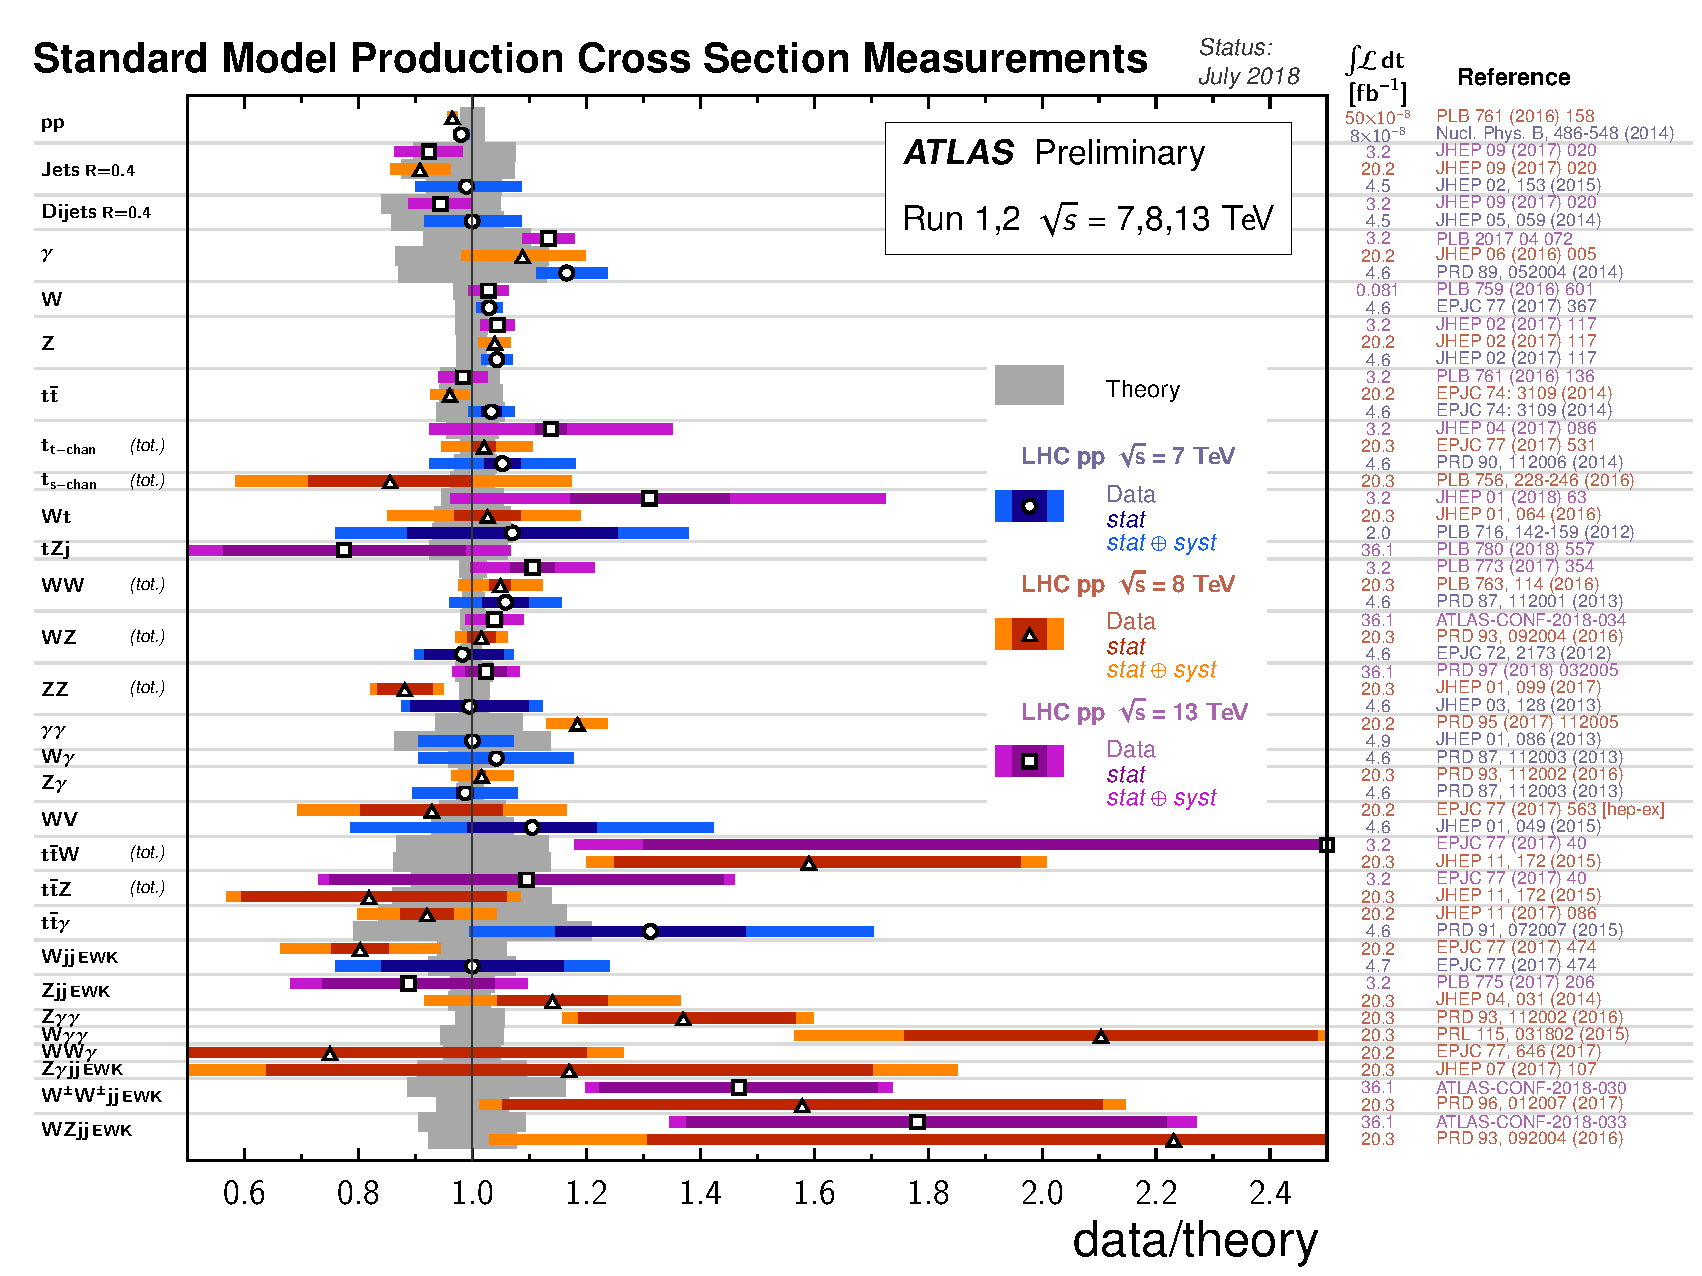
\includegraphics[width=0.6\textwidth]{sm_xsecs_atlas.pdf}
        \caption*{SM cross-sections [ATLAS, PRD 87, 112003 (2013)]}
      \end{figure}
      \begin{itemize}
        \item Currently \textbf{good agreement} between data and theory
        \item Observing deviations requires \textbf{sub-percent} accuracy
        \only<2>{
        \begin{block}{}
          {\footnotesize PDFs uncertainties is often the {\bf dominant} source of uncertainty for LHC cross-sections}
        \end{block}
        }
      \end{itemize}
    \end{column}
    \begin{column}{0.38\textwidth}
      \vspace*{-0.5cm}
      \only<2>{
      \begin{figure}
        \centering
        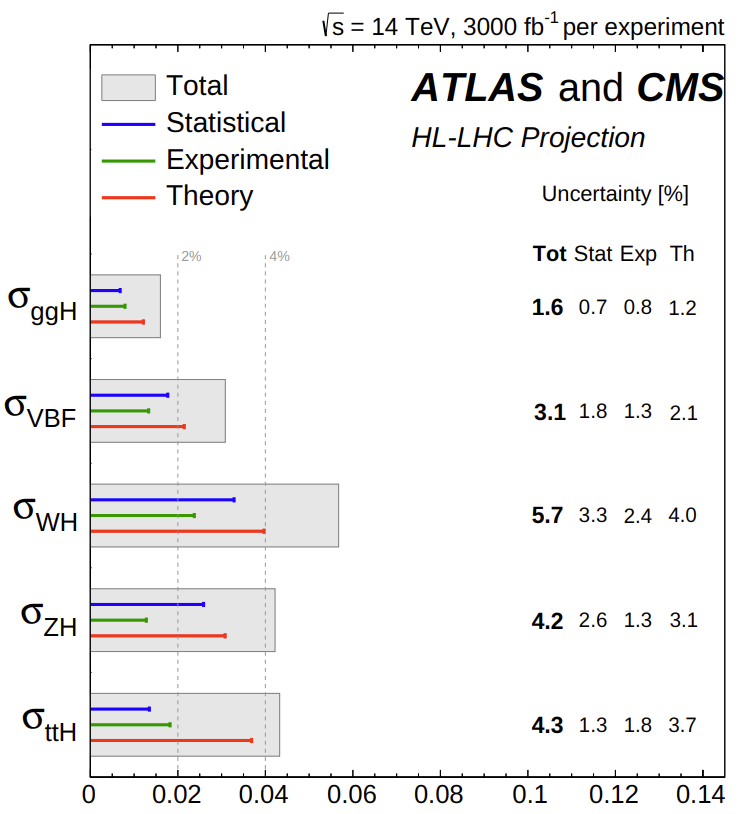
\includegraphics[width=0.7\textwidth]{hl_lhc_projection.png}
        % \only<1>{\caption*{Projection for HL-LHC [HL/HE-LHC WG2, 2019]}}
      \end{figure}
      \vspace*{-0.2cm}
      \begin{figure}
        \centering
        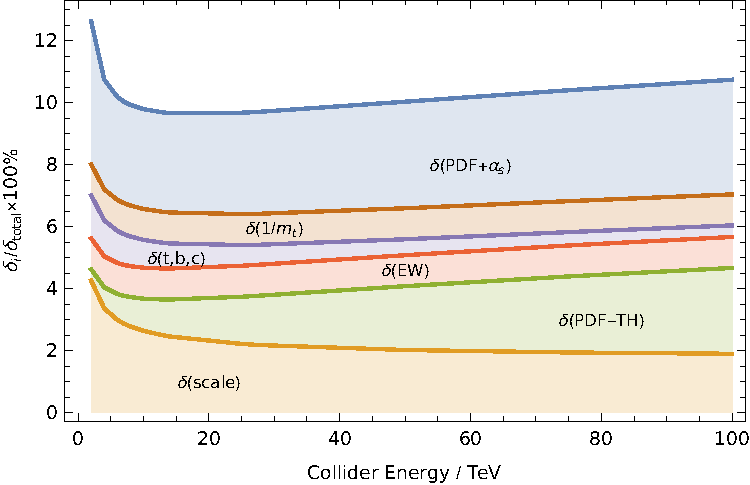
\includegraphics[width=0.7\textwidth]{sources_of_unceratinty.pdf}
        \caption*{Projection for HL-LHC [HL/HE-LHC WG2, 2019]}
      \end{figure}
      }
    \end{column}
  \end{columns}
\end{frame}


\begin{frame}[t]{Importance of faithful uncertainties}
  \begin{itemize}
    \item This years' $m_W$ determination highlights the importance of {\bf understanding all sources of uncertainty}
    \item Understand apparent {\bf discrepancies} between measurements
    \item Important that predictions are {\bf accurate}
    \item<2-> Important role for {\bf PDF uncertainties}
  \end{itemize}
  \vspace*{-0.5cm}
  \begin{columns}[t]
    \begin{column}{0.49\textwidth}
      \begin{figure}
        \centering
        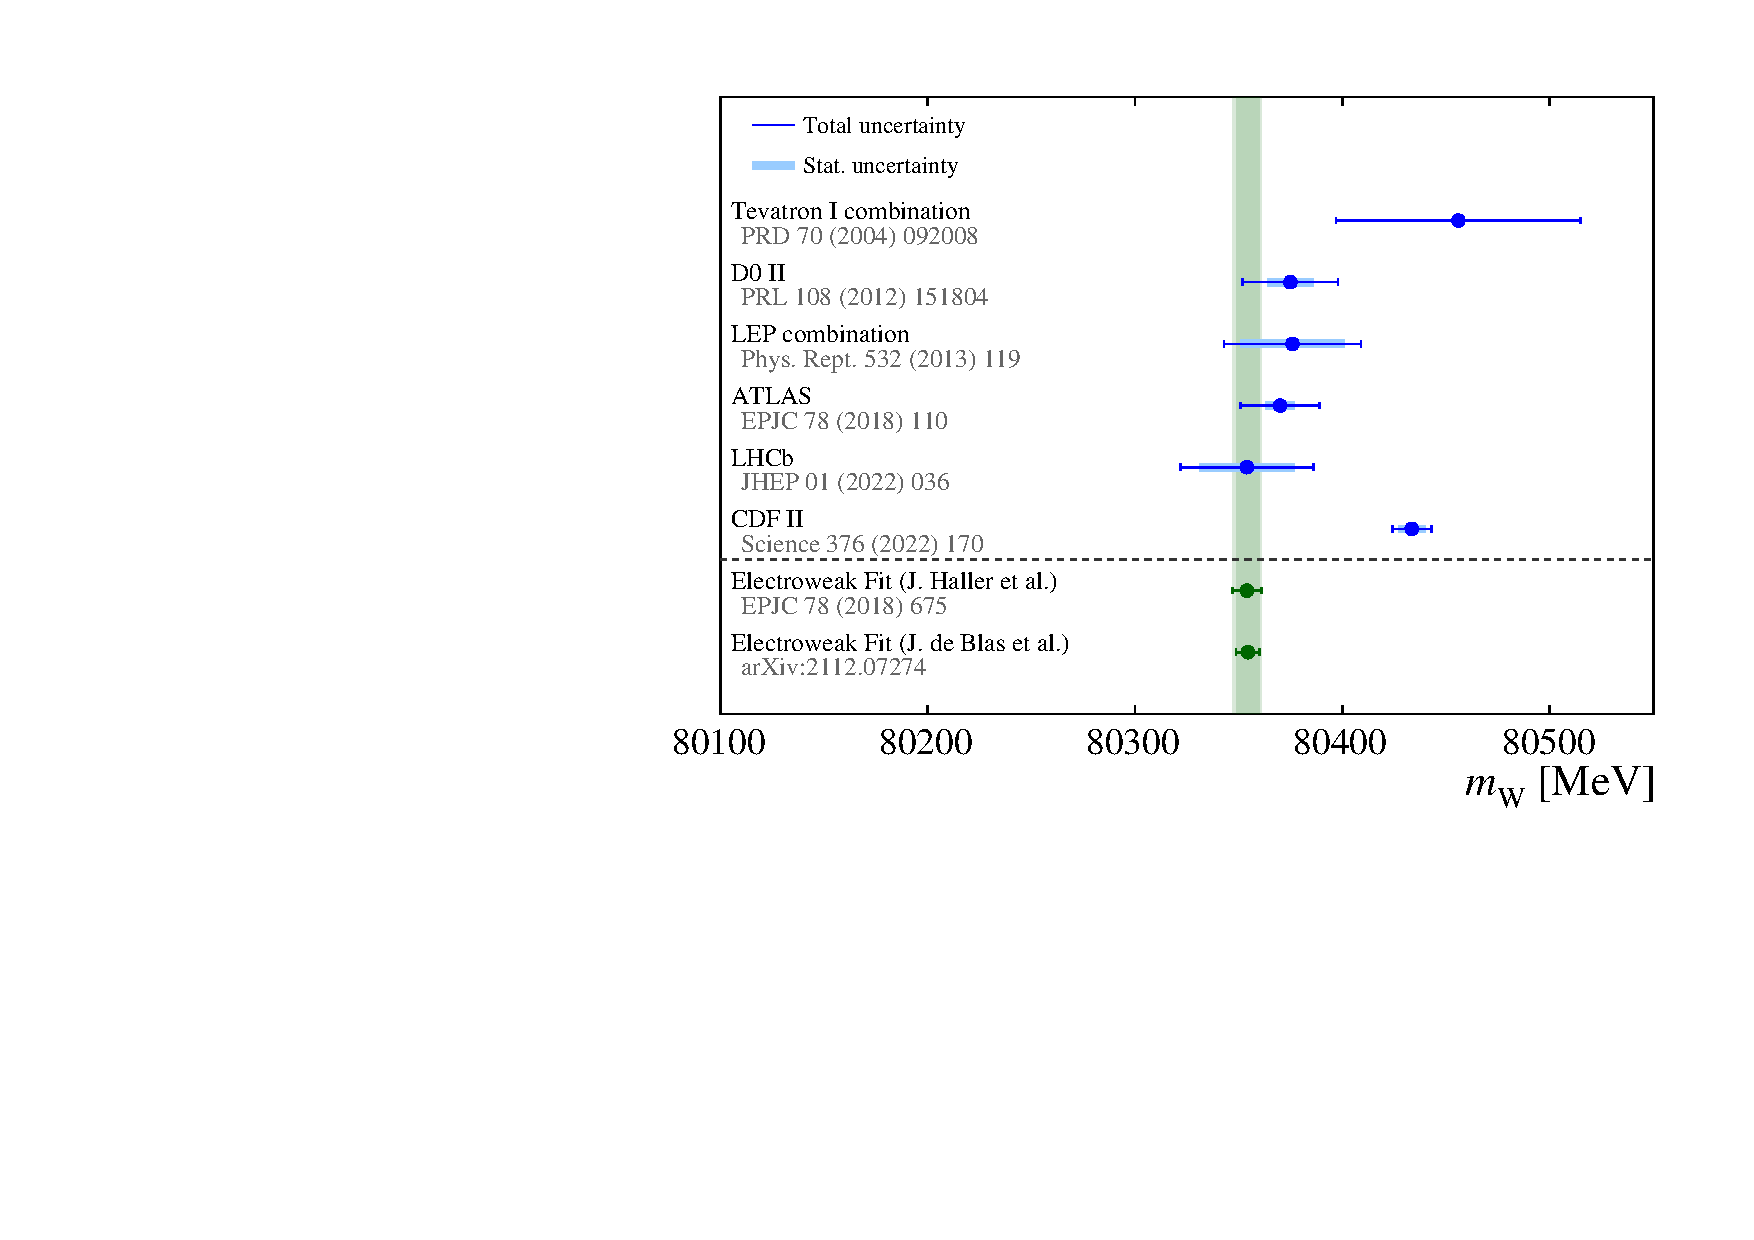
\includegraphics[width=0.7\textwidth]{lhcb_wmass.pdf}
        \caption*{SM parameters: $m_W$ [LHCb-FIGURE-2022-003]}
      \end{figure}
    \end{column}
    \begin{column}{0.49\textwidth}
      \vspace*{-1.1cm}
      \only<2->{
      \begin{figure}
        \centering
        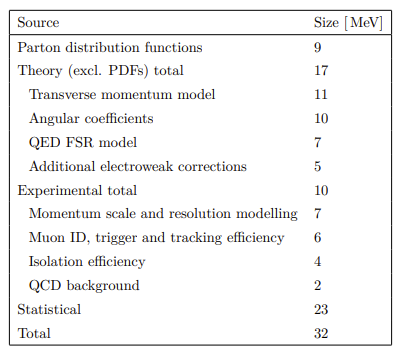
\includegraphics[width=0.7\textwidth]{lhcb_wmass_sources.png}
        \caption*{SM parameters: $m_W$ [JHEP01(2022)036]}
      \end{figure}
      }
    \end{column}
  \end{columns}
  % \only<3>{
  % \begin{center}
  %   {\bf This talk}: understanding the (robustness of) NNPDF {\bf methodological} uncertainties
  % \end{center}
  % }
\end{frame}


\begin{frame}{Status of modern PDF sets}
  \begin{columns}
    \begin{column}{0.49\textwidth}
      \begin{figure}
        \centering
        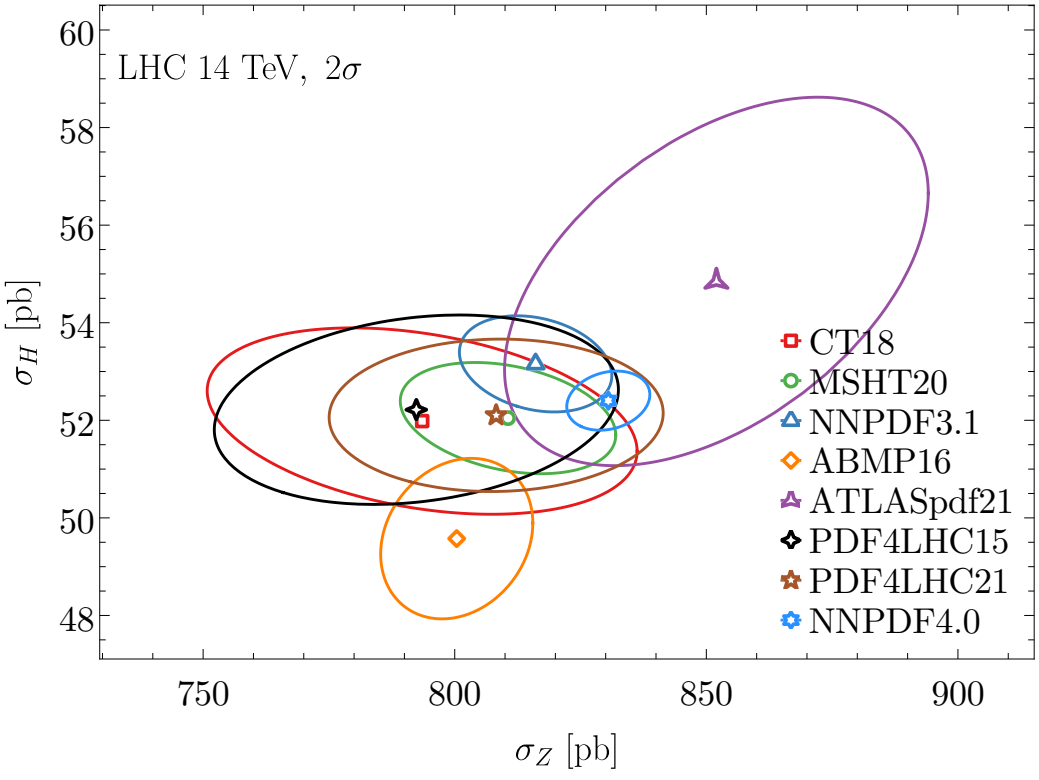
\includegraphics[width=\textwidth]{ZH_xsec_fixed.png}
        \caption*{[Snowmass (2022), 2203.13923]}
      \end{figure}
    \end{column}
    \begin{column}{0.49\textwidth}
      \begin{itemize}
        \item PDF predictions are {\bfseries consistent} but with {\bfseries different uncertainties}
        \item Ingredients of a PDF fit:
        \begin{itemize}
          \item Data
          \item Theory
          \item Methodology
        \end{itemize}
        \begin{minipage}{0.8\textwidth}
          \begin{block}{}
            {Main difference between fitting groups is the methodology}
          \end{block}
        \end{minipage}
      \end{itemize}
    \end{column}
  \end{columns}
  \only<2>{
  \begin{center}
    \textbf{``Does the NNPDF methodology produce faithful uncertainties?''}
  \end{center}
  }
\end{frame}


\begin{frame}[t]{Particularly relevant today!}
  \begin{columns}
    \begin{column}{0.49\textwidth}
      \begin{figure}
        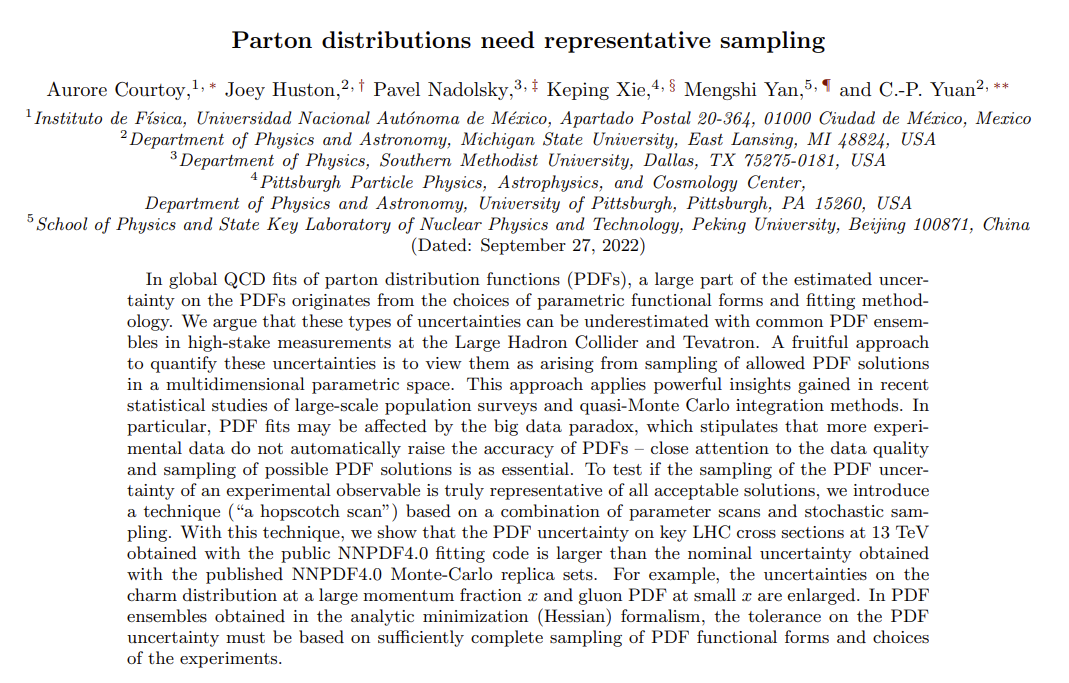
\includegraphics[width=\textwidth]{hopscotch_cover.png}
        \caption*{May 2022 [2205.10444]}
      \end{figure}
    \end{column}
    \begin{column}{0.49\textwidth}
      \begin{figure}
        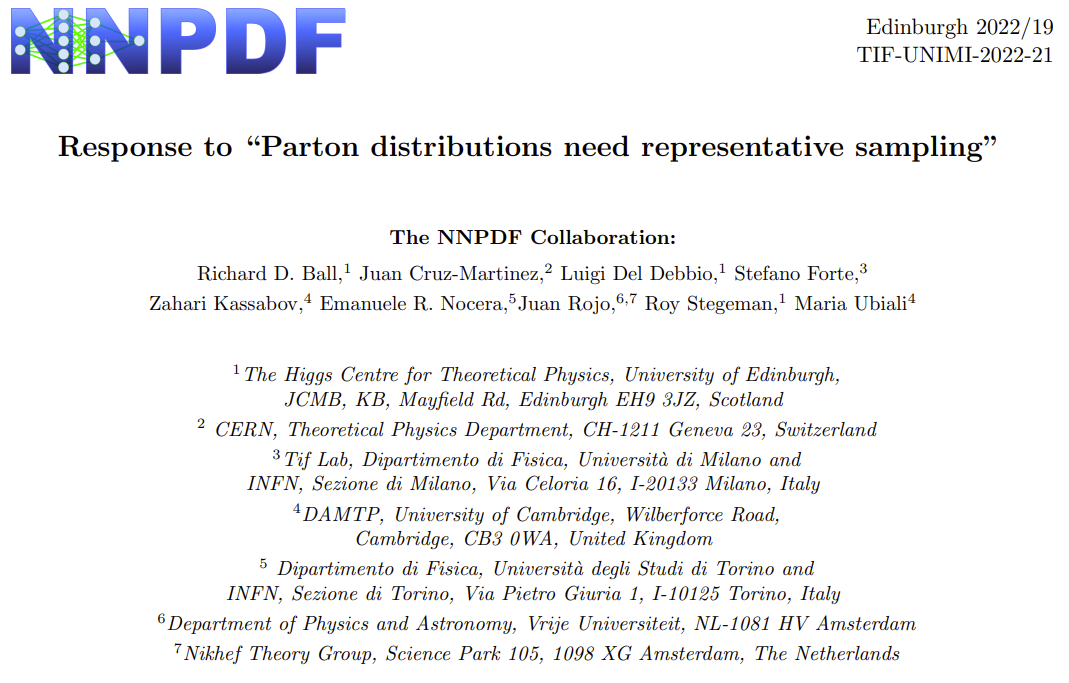
\includegraphics[width=\textwidth]{rebuttal_cover.png}
        \caption*{November 2022 [2211.12961]}
      \end{figure}
    \end{column}
  \end{columns}
\end{frame}




% Outline frame
\begin{frame}{Outline}
  \tableofcontents
\end{frame}


%%%%%%%%%%%%%%%%%%%%%%%%%%%%%%%%%%%%%%%%%%%%%%%%%%%%%%%%%%%%%%%%%%%%%%%%%%%%%%%%

{
\AtBeginSection{}
\section{NNPDF4.0}
\begin{frame}
  \begin{center}
    \usebeamerfont{section title}{NNPDF4.0}\\
    \vspace*{0.3cm} {\small 2109.02653 and 2109.02671}
  \end{center}
\end{frame}
}


\subsection{Data}


\begin{frame}[t]{PDFs from data}
  \vspace*{-0.5cm}
  \begin{columns}[T]
    \begin{column}[T]{0.49\textwidth}
      \begin{itemize}
        \item Evaluating LHC cross-sections:
          \begin{itemize}
            \itemsep 0.5em
            \item $\sigma_{ab} = \sum_{ab} {\color{red} f_a \otimes f_b} \otimes {\color{blue}\hat{\sigma}_{ab}}$
            \item PDF {\color{red}$f_a$} of flavor $a$ \\
            (non-perturbative, {\bf from data})
            \item hard-scattering matrix element {\color{blue}$\hat{\sigma}_{ab}$} \\(perturbative QCD)
            \item $\otimes$ denotes a convolution over momentum fraction $x$
          \end{itemize}
          \item PDFs {\color{red}$f_a$} depends only on $x$ and $Q^2$
          \item Other kinematic variables in {\color{blue}$\hat{\sigma}$}
      \end{itemize}
      \vspace*{0.3cm}
      \only<2->{
      {\bf The problem}
      \begin{itemize}
        \item Given a dataset $D$, determine $p(f|D)$ in the space of PDFs $f:[0,1]\to \mathbb{R}$
        \item PDFs are multivariate probability distributions in {\bf infinite dimensional} space
        \item However data is {\bf discrete}
        % \item Problem is undetermined: solution depends on {\bf assumptions}
      \end{itemize}
      }
    \end{column}
    \begin{column}{0.49\textwidth}
      \begin{center}
        \only<-2>{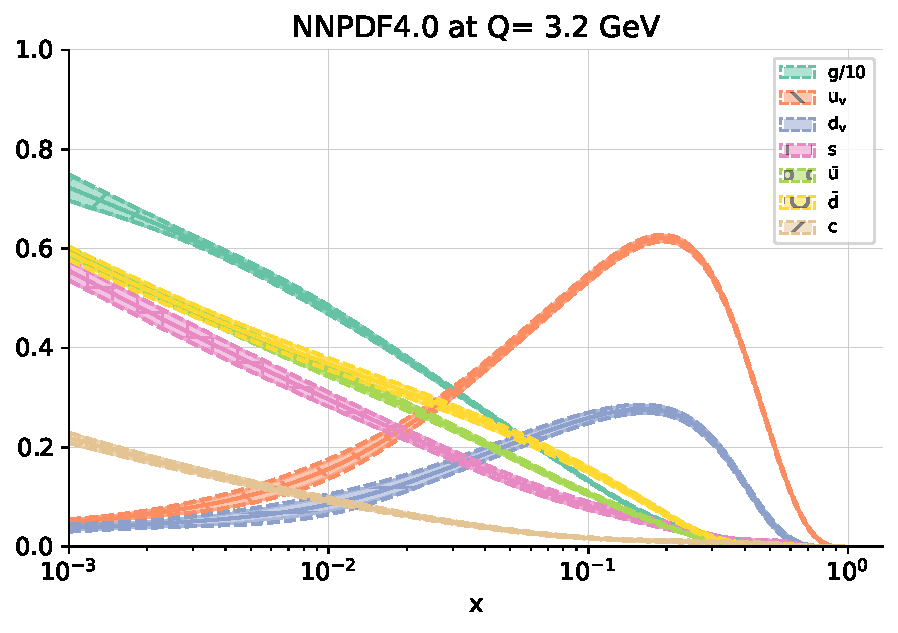
\includegraphics[width=\textwidth]{Qs0_plot_flavours.pdf}}
      \end{center}
    \end{column}
  \end{columns}
\end{frame}


\begin{frame}[t]{Data in NNPDF4.0}
  \begin{center}
    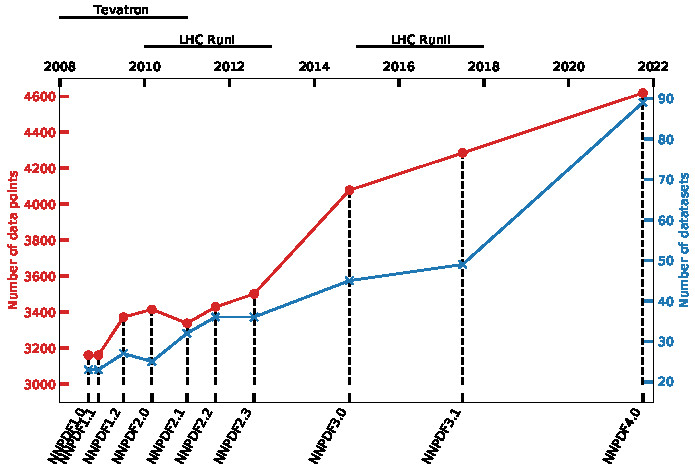
\includegraphics[width=0.7\textwidth]{NNPDF_data_history.pdf}
  \end{center}
  Better data $\rightarrow$ higher precision and accuracy
\end{frame}


\begin{frame}[t]{Data in NNPDF4.0}
  \begin{columns}
      \column{0.7\linewidth}
          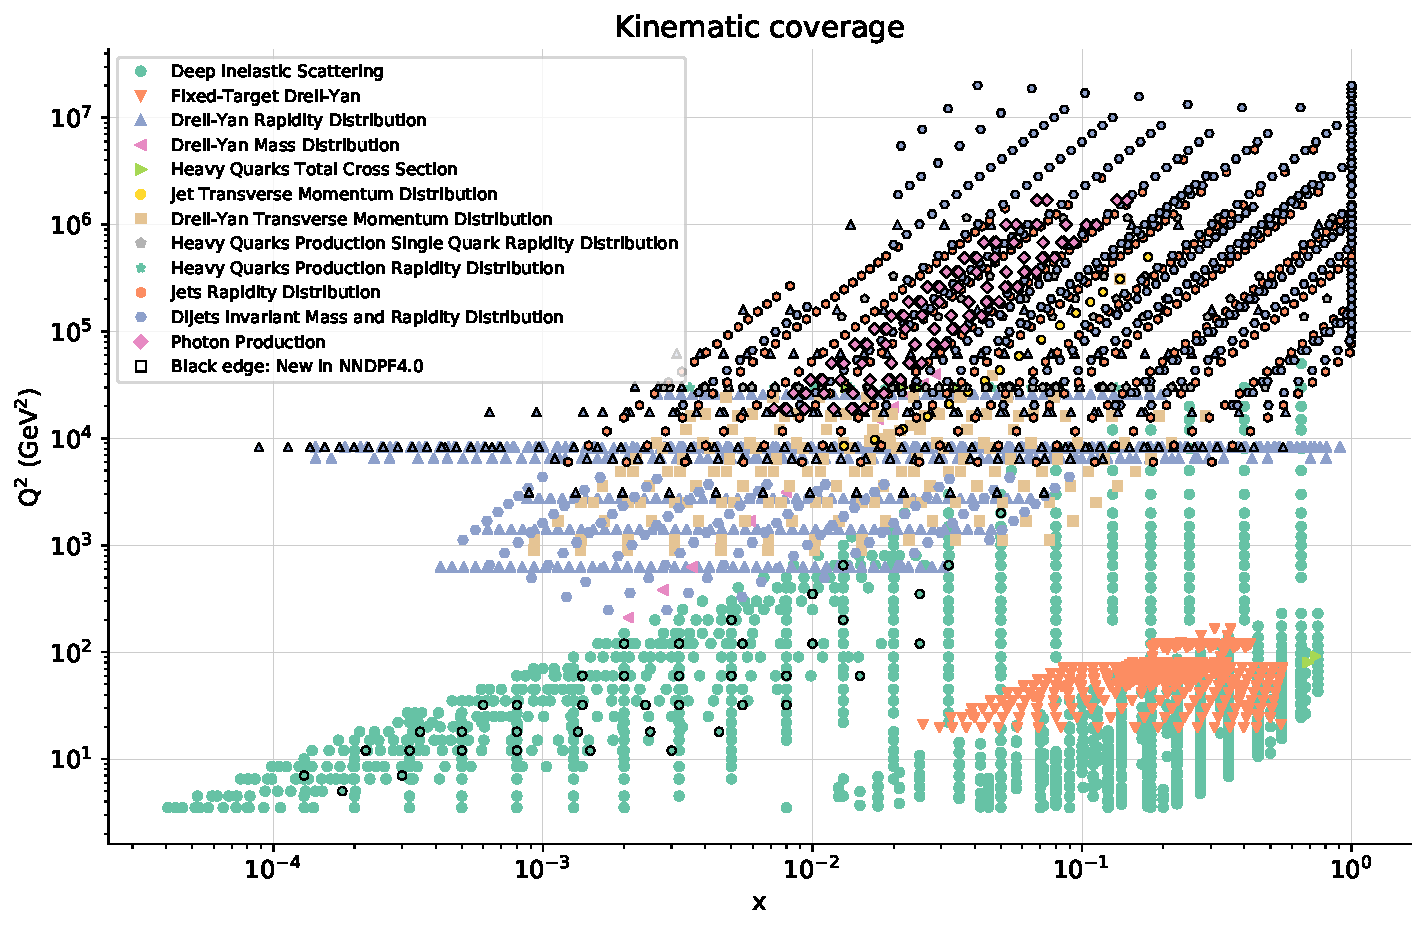
\includegraphics[width=1.0\textwidth]{Markers0_plot_xq2}
      \column{0.3\linewidth}
          More than 4000 datapoints\\
          and 13 processes!\\
          \vspace*{1em}
          New processes:
          \begin{itemize}
              \item direct photon
              \item single top
              \item dijets
              \item W+jet
              \item DIS jet
          \end{itemize}
  \end{columns}
\end{frame}


\subsection{Methodology}


\begin{frame}[t]{The NNPDF approach: probabilities in a space of function}
  \begin{columns}[T]
    \begin{column}[T]{0.49\textwidth}
      Data is fully defined by central values $\mu_i$ and covariance matrix $\operatorname{cov}_{ij}$
      \begin{enumerate}
        \item Generate $N_{\rm rep}$ {\color{datasamplegreen} Monte Carlo data} ``replicas'' $\hat{\mu}_i$ such that as $N_{\rm rep}\to \infty$ \\
        $\mu_i = \frac{1}{N_{\rm rep}}\sum_{i=1}^{N_{\rm rep}} \hat{\mu}_i$\\
        $\operatorname{cov}_{ij} = \operatorname{cov}[\hat{\mu}_i, \hat{\mu}_j]$
        \item Perform a {\color{red} PDF fit} to each replica
        \item Compute observables $X$ and their uncertainties\\
        $\left\langle X\left[f\right]\right\rangle=\frac{1}{N_{\rm rep}} \sum_{r=1}^N X\left[f^{(r)}\right]$\\
        $\operatorname{Var}\left[X\left[f\right]\right] = \frac{1}{N_{\rm rep}} \sum_{r=1}^{N_{\rm rep}}\left(X\left[f^{(r)}\right]-\left\langle X\left[f\right]\right\rangle\right)^2$
      \end{enumerate}
      \vspace*{0.3cm}
      \only<2>{
      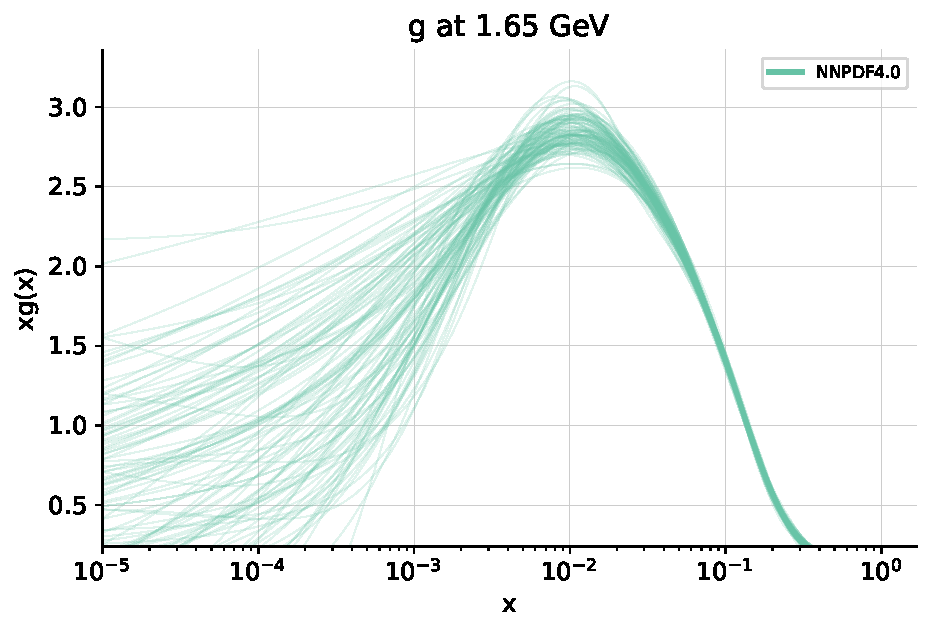
\includegraphics[width=0.49\textwidth]{replicas_g.pdf}
      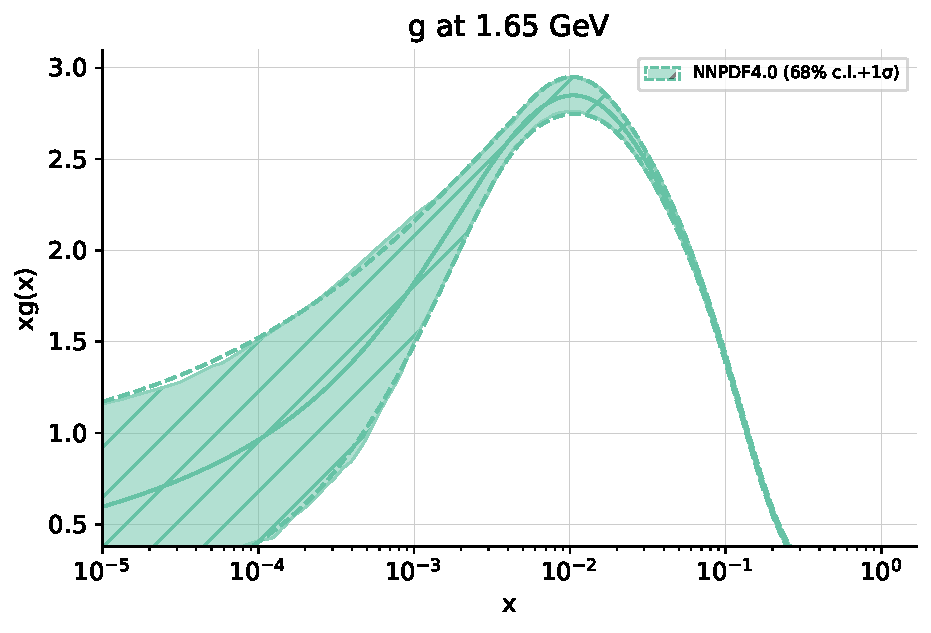
\includegraphics[width=0.49\textwidth]{band_g.pdf}
      }
    \end{column}
    \begin{column}{0.49\textwidth}
      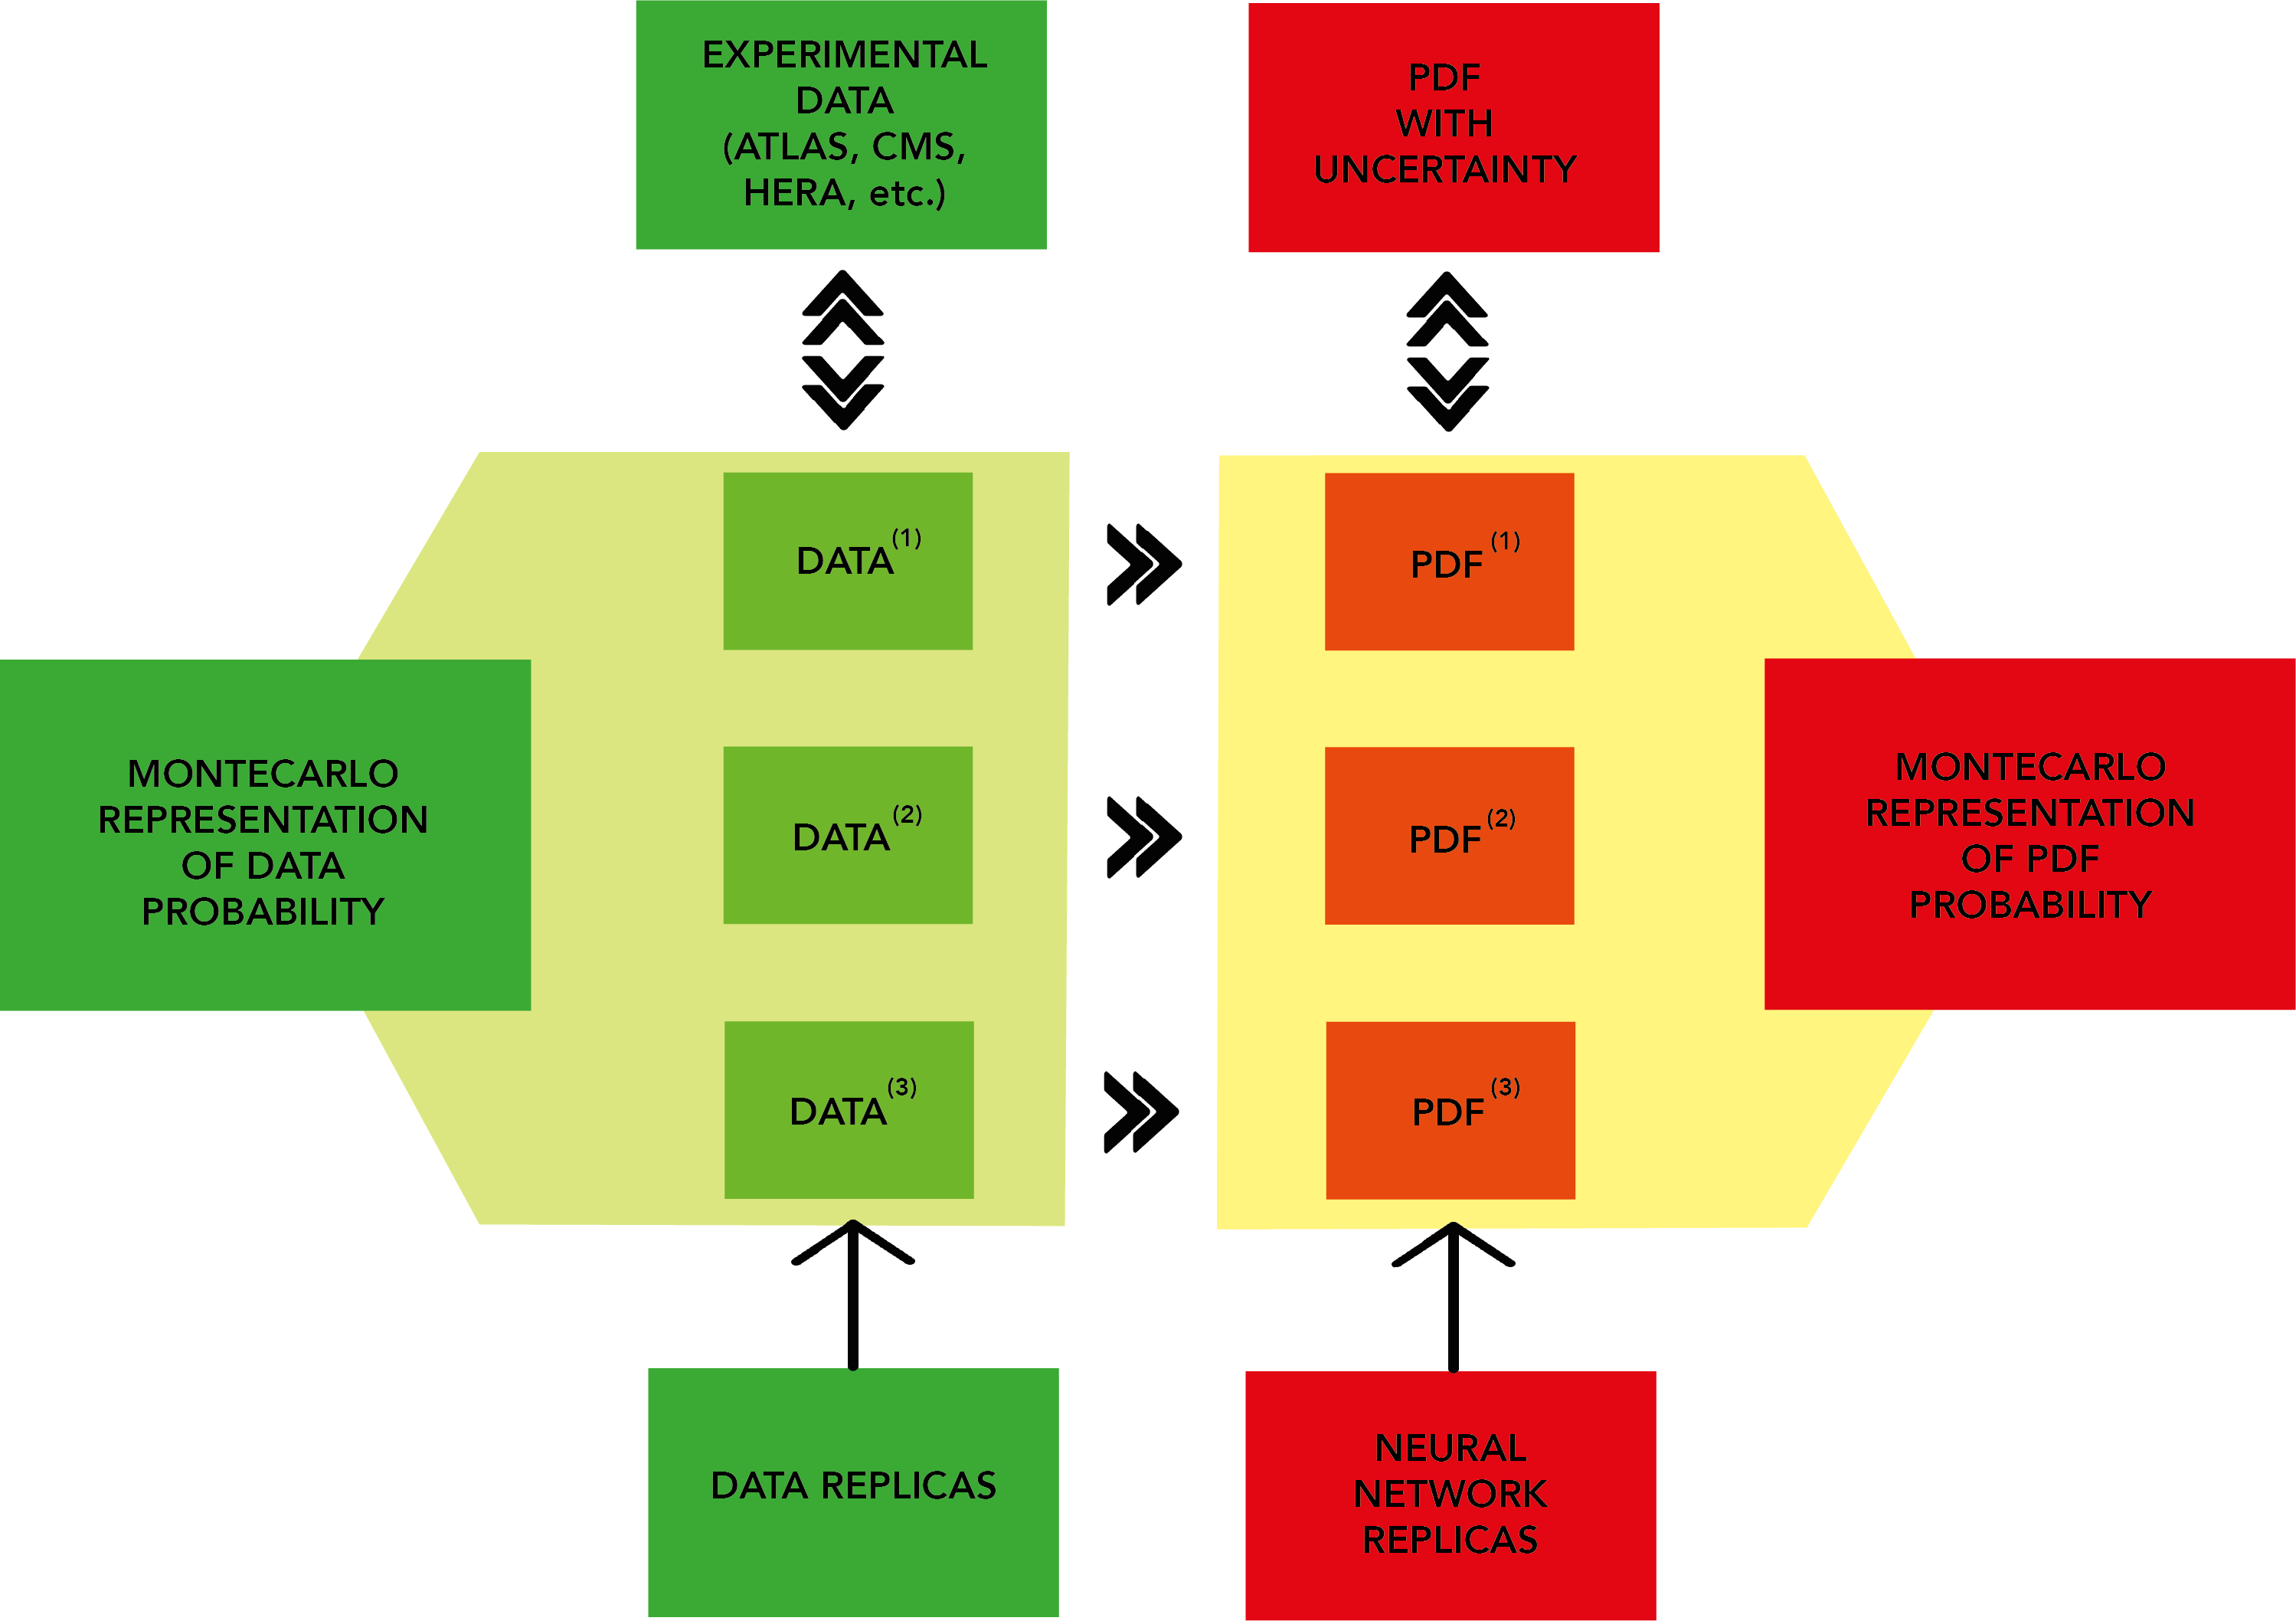
\includegraphics[width=\textwidth]{nnpdf_strat.png}
    \end{column}
  \end{columns}
\end{frame}


\begin{frame}[t]{The NNPDF approach: an importance sampling}
  \begin{itemize}
    \item Importance sampling produces Gaussian posterior distribution
    \item All replicas equally likely
  \end{itemize}
  \begin{center}
    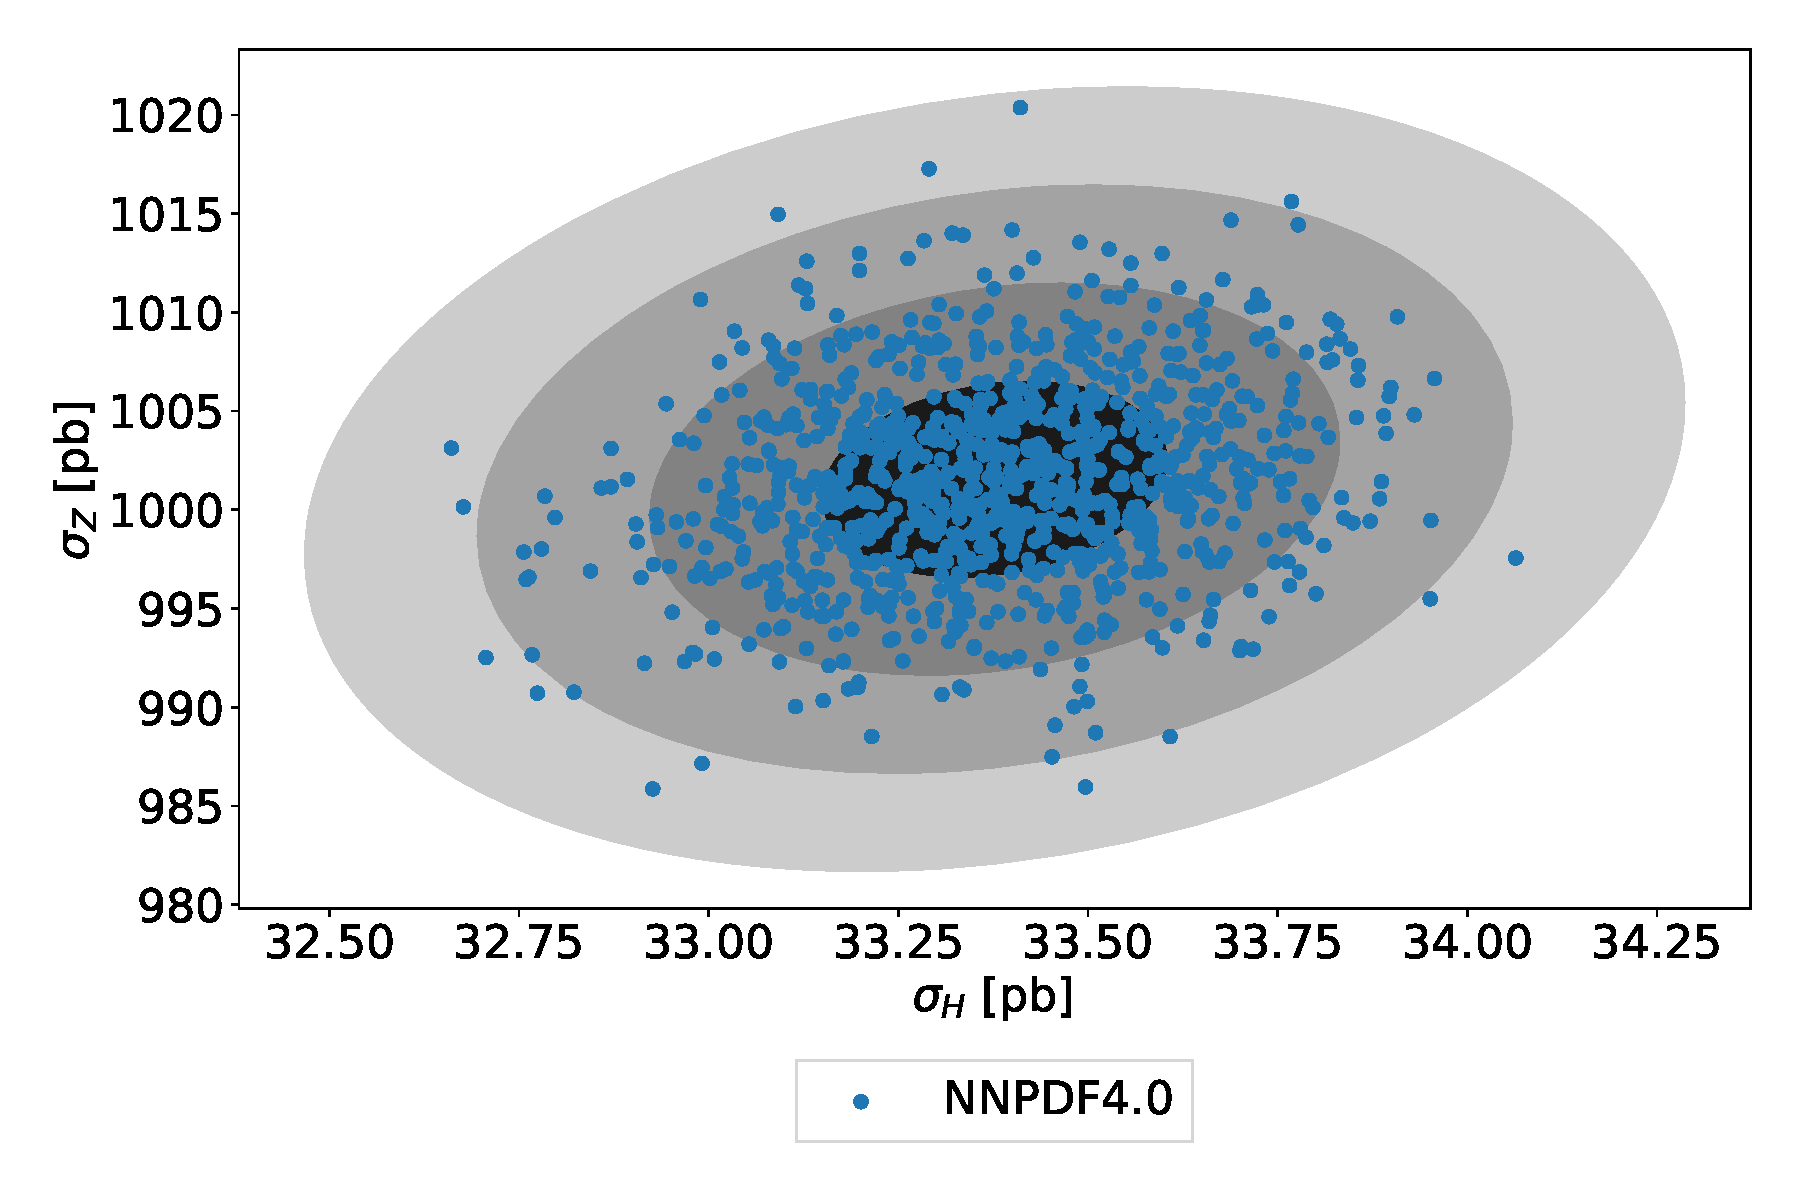
\includegraphics[width=0.5\textwidth]{nnpdf40_dist.pdf}
  \end{center}
  \only<2>{
  \begin{center}
    {\bf How did we obtain this distribution?}
  \end{center}
  }
\end{frame}



\begin{frame}[t]{Parametrization}
  \begin{columns}[T]
      \begin{column}{0.48\textwidth}
        Neural network: universal interpolator
        \vspace*{0.3cm}
        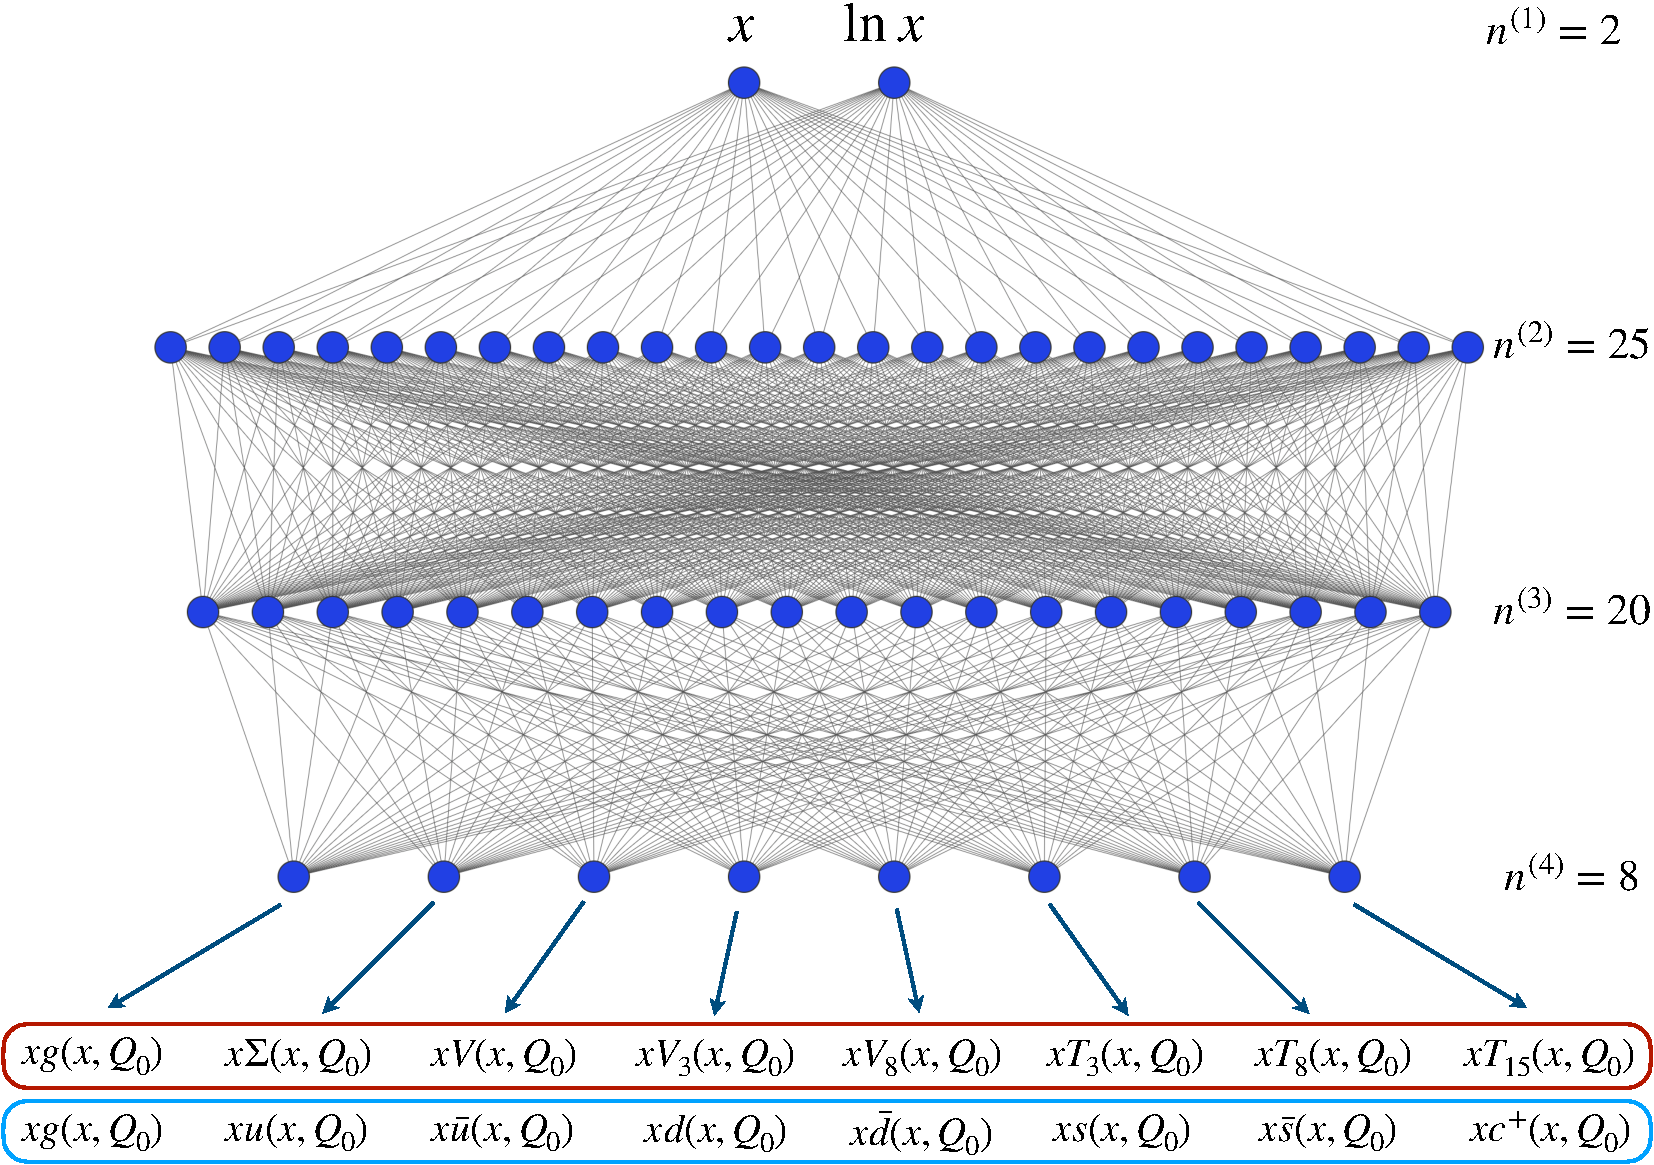
\includegraphics[width=1.0\textwidth]{NNarch}
        \begin{equation*}
            f_{i}\left(x, Q_{0}\right)=x^{-\alpha_{i}}(1-x)^{\beta_{i}} \mathrm{NN}_{i}(x)
        \end{equation*}
      \end{column}
      \begin{column}{0.48\textwidth}
        Physical constraints:
        \begin{itemize}
            \item PDF positivity [JHEP 11 (2020)]
            \item Integrability of nonsinglet distributions (Gottfried sum rules)
        \end{itemize}
        \vspace*{0.3cm}
        \begin{itemize}
          \item Train by minimizing $\chi^2$ loss function comparing data to prediction\\
          % \item Remember $\sigma_{ab} = \sum_{ab} {\color{red} f_a \otimes f_b} \otimes {\color{blue}\hat{\sigma}_{ab}}$
          % \begin{itemize}
          %   \item Experimental data
          %   \item Model/parametrization
          %   \item Theory: ${\color{blue}\hat{\sigma}_{ab}}$ in precomputed grids
          % \end{itemize}
        \end{itemize}
      \end{column}
  \end{columns}
\end{frame}


% \begin{frame}{The NNPDF4.0 model}{See  \href{https://arxiv.org/pdf/1907.05075}{\color{blue} EPJ\,C79\,(2019)\,676}}
%   \begin{figure}[t]
%     \centering
%     \resizebox{0.8\textwidth}{!}{%
%       \begin{tikzpicture}[node distance = 1.0cm]\scriptsize
%       % Input node
%       \node (xinput) {$\{\mathrm{xgrid}_n\}$};

%       % PDF basis
%       \coordinate [right = 1.5cm of xinput] (NNghost) {};
%       \node[fitted, above = 1.0cm of NNghost, minimum width=1.7cm, minimum height=0.7cm] (pdf) { Neural Net};
%       \node[fitted, below = 1.0cm of NNghost, minimum width=1.7cm, minimum height=0.7cm] (preproc) { $x^{\alpha}$ $(1-x)^{\beta}$};
%       \node[above = 0.6cm of pdf, minimum width=1.7cm, minimum height=0.3cm] (fform)
%       {\color{red} {\fontsize{10pt}{0}\selectfont $\mathrm{PDF}=Ax^\alpha(1-x)^\beta \mathrm{NN}(x,\log x)$} };

%       % PDF production
%       \node[operations, fill=violet!40, minimum width=1.2cm, minimum height=0.7cm, right = 1.5cm of NNghost]
%           (fitbasis) {$\overline{\mathrm{PDF}}_n$};
%       \node[operations, fill=violet!40, minimum width=1.2cm, minimum height=0.7cm, right = 0.6cm of fitbasis]
%           (normalizer) {normalization};

%       % PDFs 1 to n
%       \node[right = 0.9cm of normalizer] (pdfdots) {\vdots};
%       \node[above = 0.7cm of pdfdots] (pdf1) {PDF$_1$};
%       \node[below = 0.7cm of pdfdots] (pdfn) {PDF$_n$};

%       % Convolutions 1 to n
%       \node[right = 0.2cm of pdf1] (conv1) {$\otimes$};
%       \node[right = 0.2cm of pdfn] (convn) {$\otimes$};
%       \node at ($(conv1)!0.5!(convn)$) (convdots) {$\otimes$};

%       % FK Tables 1 to n
%       \node[blue, right = 0.6cm of conv1] (f1) {$\hat{\sigma}_1$};
%       \node[blue, right = 0.6cm of convn] (fn) {$\hat{\sigma}_n$};
%       \node[blue] at ($(f1)!0.5!(fn)$) (fd) {\vdots};
%       \draw[draw=blue, rounded corners] ($(f1.north west)+(-0.1, 0.2)$) rectangle ($(fn.south east)+(0.1,-0.2)$);
%           \node[above = 0.6cm of f1] (theory) {Theory};
%           \coordinate [above = 0.2cm of f1] (theoryarrow) {};

%       % Observables
%       \node[right = 0.5 cm of f1] (o1) {$\mathcal{O}_{1}$};
%       \node[right = 0.5 cm of fn] (on) {$\mathcal{O}_{n}$};
%       \node at ($(o1)!0.5!(on)$) (od) {\vdots};
%       \node[above = 0.9cm of o1] (observables) {Observables};
%       \coordinate [above = 0.2cm of o1] (observablearrow) {};

%       % Tr/Vl split
%       \node[operations, right = 0.5cm of od, minimum width = 1.2cm, text width=1cm, minimum height=0.7cm]
%       (trvl) {Tr/Vl split};
%       \coordinate [right = 1.0cm of trvl] (ending) {};
%       \path let \p1 = (ending), \p2 = (pdf)
%           in node at (\x1,\y2) [n3py, minimum width = 1.2cm, minimum height=0.7cm] (tr) {$\chi^{2}_\text{tr}$};
%       \path let \p1 = (ending), \p2 = (preproc)
%           in node at (\x1,\y2) [n3py, minimum width = 1.2cm, minimum height=0.7cm] (vl) {$\chi^{2}_\text{vl}$};

%       % Arrows!
%       \draw[myarrow] (xinput) -- (pdf);
%       \draw[myarrow] (xinput) -- (preproc);
%       \draw[myarrow] (pdf) -- (fitbasis);
%       \draw[myarrow] (preproc) -- (fitbasis);
%       \draw[myarrow] (fitbasis) -- (normalizer);

%       \draw[myarrow] (pdf1) -- (conv1);
%       \draw[myarrow] (pdfn) -- (convn);
%       \draw[myarrow] (conv1) -- ($(f1.west)-(0.2,0.0)$) ;
%       \draw[myarrow] (convn) -- ($(fn.west)-(0.2,0.0)$) ;
%       \draw[myarrow] ($(f1.east)+(0.2,0.0)$) -- (o1);
%       \draw[myarrow] ($(fn.east)+(0.2,0.0)$) -- (on);

%       \draw[myarrow] (trvl) -- (tr);
%       \draw[myarrow] (trvl) -- (vl);

%       \draw[myarrow] (theory) -- (theoryarrow);
%       \draw[myarrow] (observables) -- (observablearrow);

%       % Braces
%       \draw[decorate, decoration={brace}, thick] (pdfn.south west) -- (pdf1.north west);
%       \draw[decorate, decoration={brace},thick] (o1.north east) -- (on.south east);
%       \end{tikzpicture}
%     }
%   \end{figure}
%   % \textbf{Main changes:}
%   \vspace*{2em}
%   \begin{itemize}
%       \item Modular \texttt{Python} codebase
%       \item Freedom to use external libraries (default: \texttt{TensorFlow})
%       % \item Modularity $\Rightarrow$ ability to vary all aspects of the methodology
%   \end{itemize}
% \end{frame}


\begin{frame}[t]{Training the neural network}
  \begin{itemize}
    \item Optimize using a gradient descent algorithm
    \item NN should generalize the underlying law, but if trained to long noise is fitted
  \end{itemize}
  \begin{columns}[T]
    \begin{column}[T]{0.49\textwidth}
      Cross-validation
      \begin{itemize}
        \item Divide data into {\color{blue} training} and {\color{orange} validation}
        \item Minimize training $\chi^2$
        \item {\color{red} Stop} if {\color{orange} validation} $\chi^2$ no longer improves
      \end{itemize}
      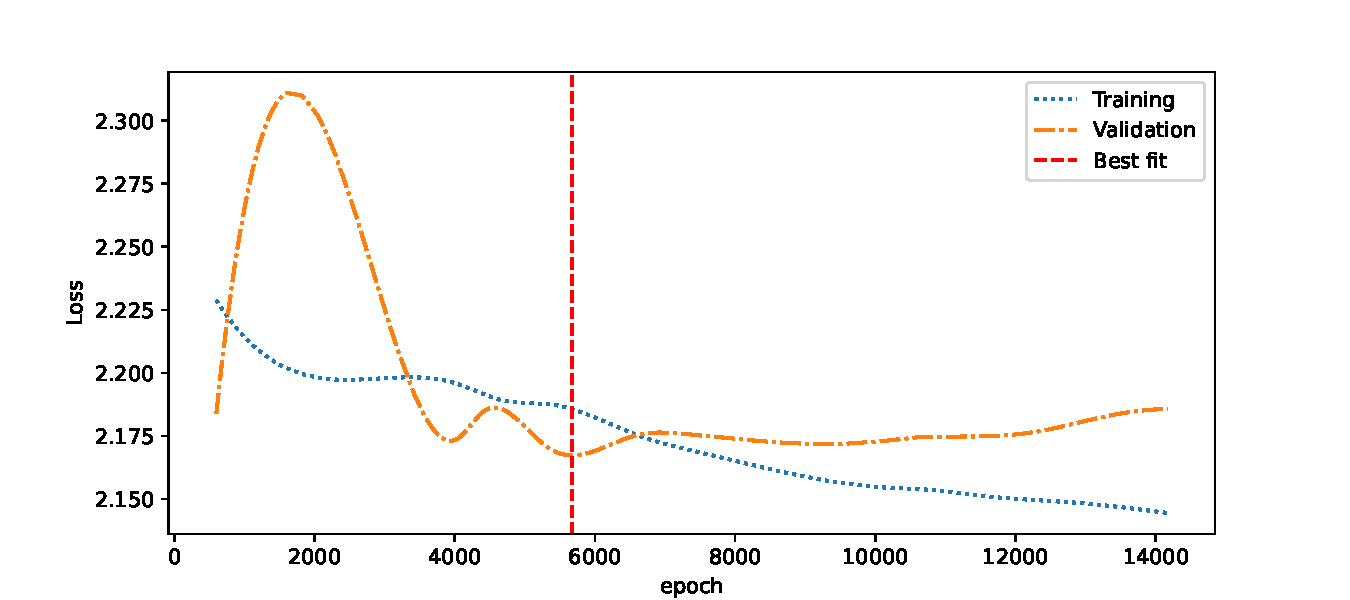
\includegraphics[width=0.9\textwidth]{trvl.pdf}
    \end{column}
    \begin{column}{0.49\textwidth}
      \begin{figure}
        \centering
        \resizebox{\columnwidth}{!}{
        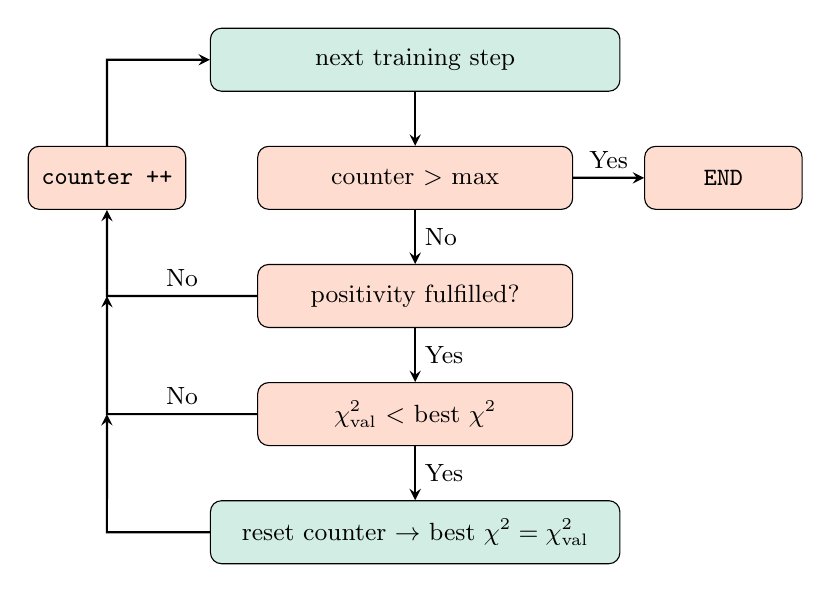
\begin{tikzpicture}[node distance = 1.5cm, scale=0.1]\small
            \definecolor{vp1}{RGB}{102,194,165}
            \definecolor{vp2}{RGB}{252,141,98}
            % Middle column
            \node (init) [roundtext, fill=vp1!30, minimum width=5.2cm] {next training step};
            \node (ccheck) [roundtext, fill=vp2!30, minimum width=4cm, minimum height=0.8cm, below of = init] {counter
                $>$ max};
            \node (pcheck) [roundtext, fill=vp2!30, minimum width=4cm, minimum height=0.8cm, below of = ccheck]
                {positivity fulfilled?};
            \node (xcheck) [roundtext, fill=vp2!30, minimum width=4cm, minimum height=0.8cm, below of = pcheck]
                {$\chi^2_\text{val}$ $<$ best $\chi^2$};
            \node (reset) [roundtext, fill=vp1!30, minimum width=5.2cm, below of = xcheck] {reset counter $\rightarrow$  best
                $\chi^2 = \chi^2_\text{val}$};Q

            % Off-center nodes
            \node (cplus) [roundtext, fill=vp2!30, left = 0.9cm of ccheck]
                {\ttfamily counter ++};
            \node (end) [roundtext, fill=vp2!30, right = 0.9cm of ccheck]
                {\ttfamily END};

            % Coordinates
            \coordinate[above of = cplus] (li);
            \coordinate[below of = cplus] (lp);
            \coordinate[below of = lp] (lx);
            \coordinate[below of = lx] (lr);


            % Arrows center
            \draw[myarrow] (init) -- (ccheck);
            \draw[myarrow] (ccheck) -- node[right] {No} (pcheck);
            \draw[myarrow] (pcheck) -- node[right] {Yes}(xcheck);
            \draw[myarrow] (xcheck) -- node[right] {Yes}(reset);

            % Arrows off-center
            \draw[myarrow] (ccheck) --  node[above] {Yes} (end);

            \draw[myarrow] (reset) -- (lr) -- (lx);
            \draw[myarrow] (xcheck) -- node[above] {No} (lx) -- (lp);
            \draw[myarrow] (pcheck) --  node[above] {No} (lp) -- (cplus);
            \draw[myarrow] (cplus) -- (li) -- (init);
        \end{tikzpicture}
        }
      \end{figure}
    \end{column}
  \end{columns}
\end{frame}


\begin{frame}[t]{Verify the importance sampling assumption}
  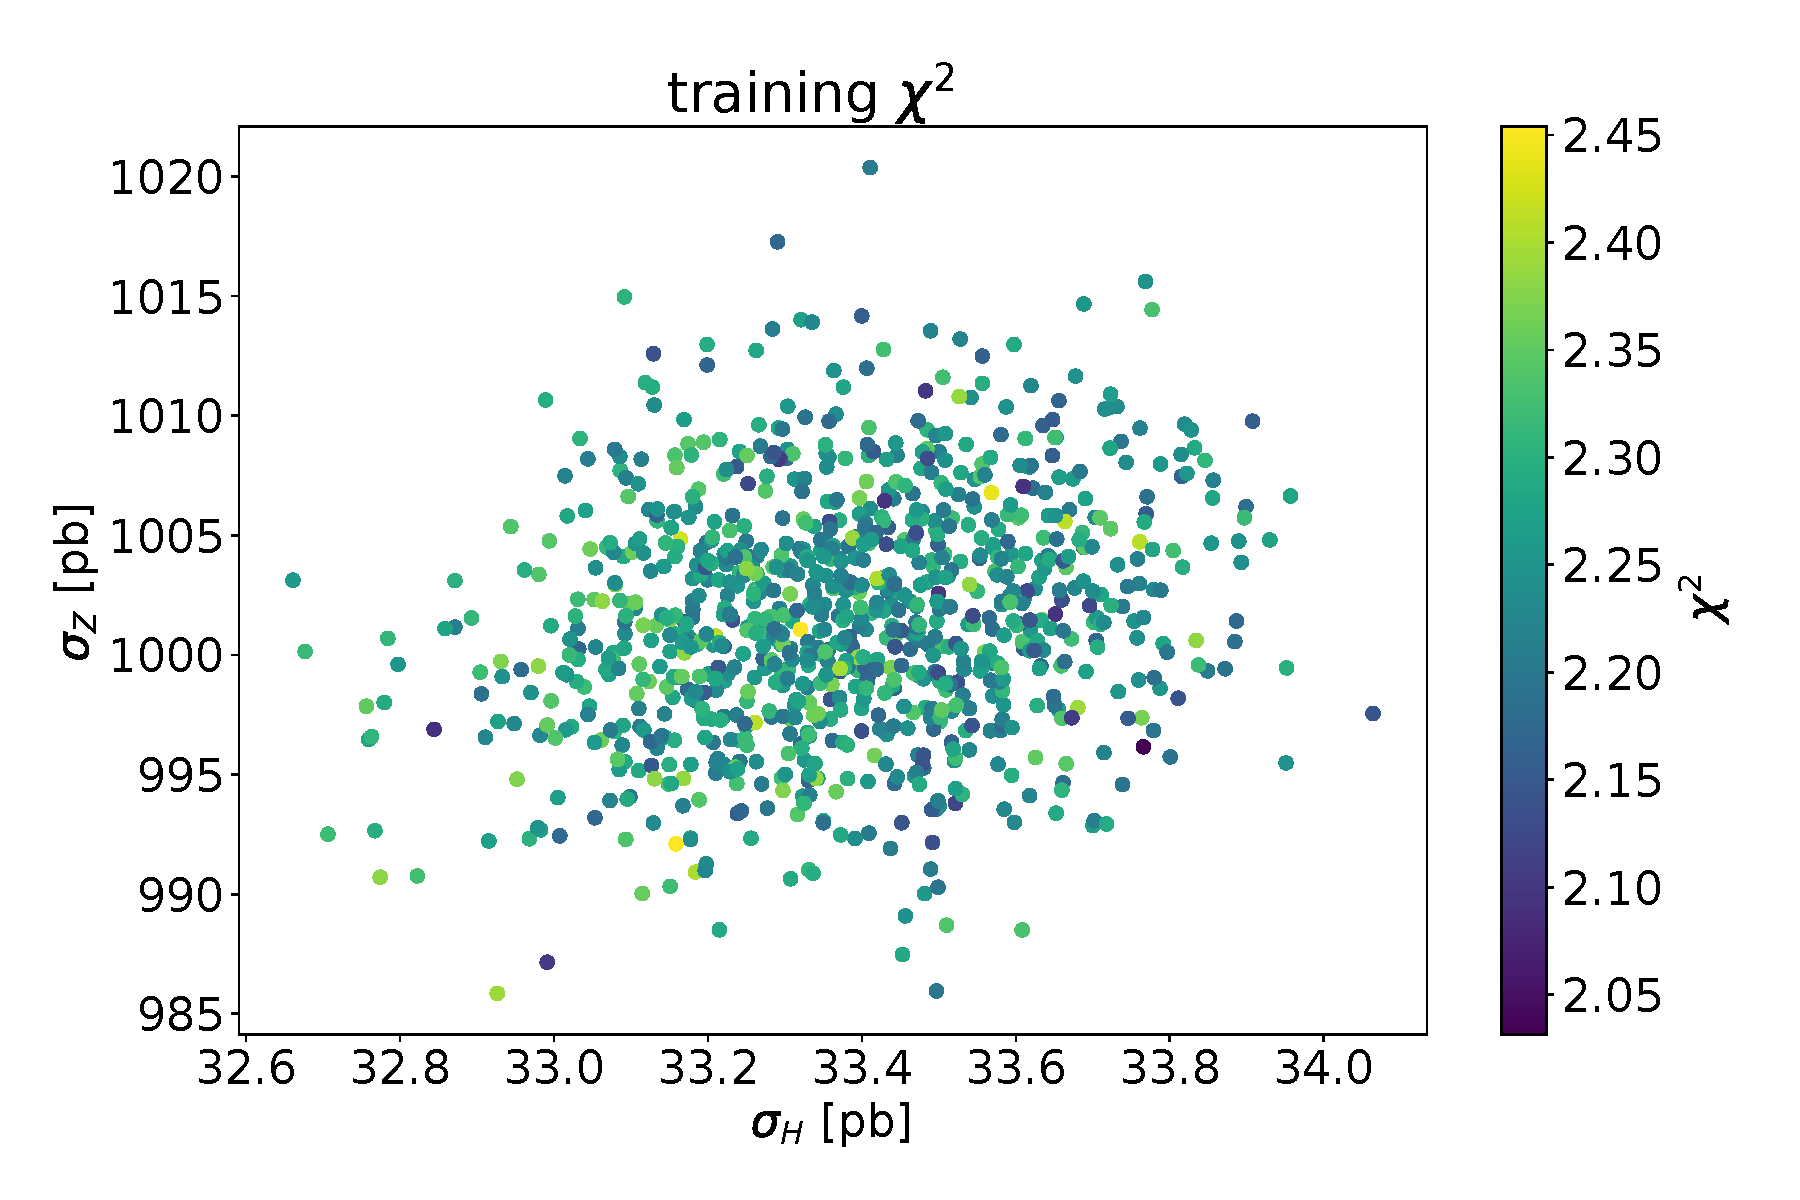
\includegraphics[width=0.49\textwidth]{chi2_training_chi2.pdf}
  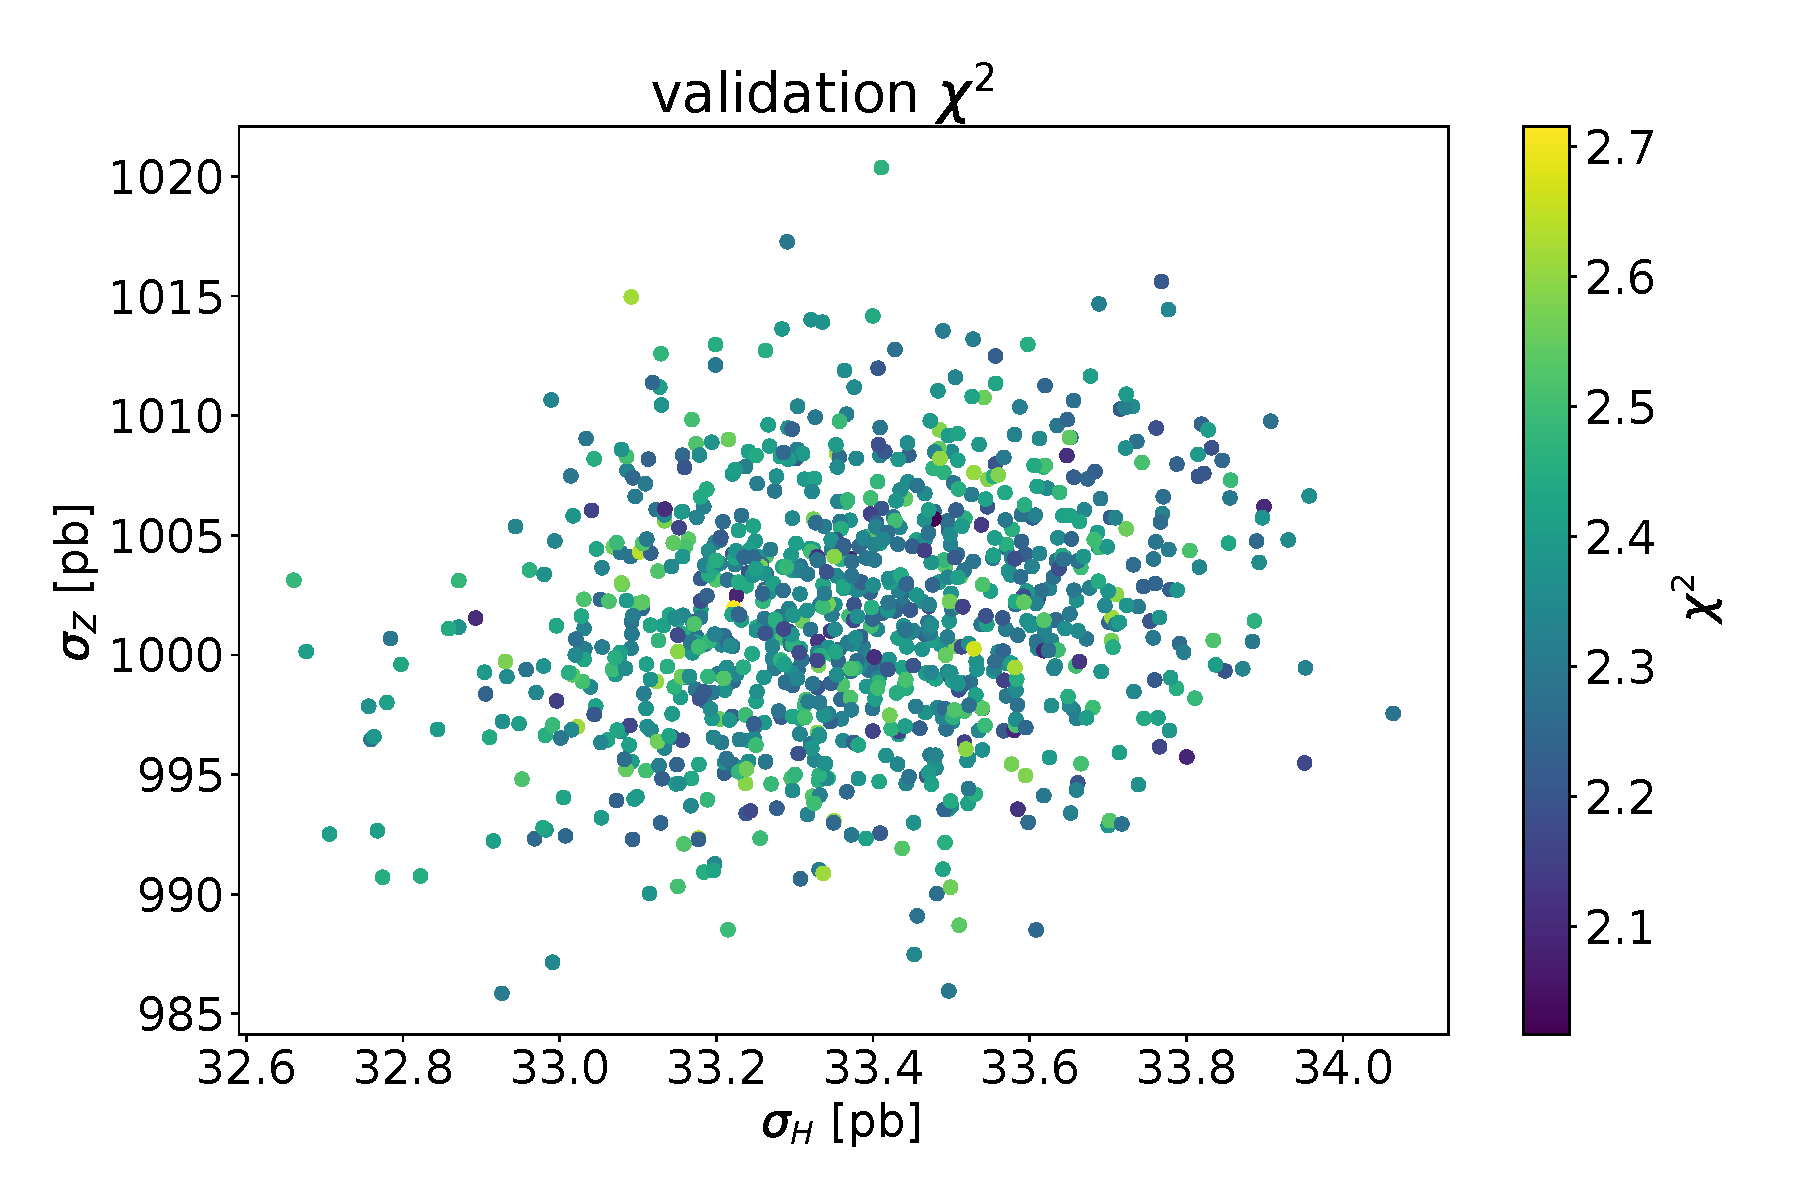
\includegraphics[width=0.49\textwidth]{chi2_validation_chi2.pdf}
  \begin{itemize}
    \item All PDF replicas are fitted equally well to their data replica
    \item Thus outliers correspond to unlikely data replicas
  \end{itemize}
\end{frame}


\begin{frame}[t]{Automated model selection}
  NNPDF aims to minimize sources of bias in the PDF:
  \begin{itemize}
    \item Functional form $\rightarrow$ Neural Network
    \item Model parameters $\rightarrow$ ?
  \end{itemize}
\end{frame}


\begin{frame}[t]{Automated model selection}
  NNPDF aims to minimize sources of bias in the PDF:
  \begin{itemize}
      \item Functional form $\rightarrow$ Neural Network
      \item Model parameters $\rightarrow$ \textbf{Hyperoptimization}
  \end{itemize}
    \begin{columns}
        \begin{column}{0.48\textwidth}
            Scan over thousands of hyperparameter combinations and select the best one \\
            \vspace*{0.8em}
            {\bf k-fold cross-validation}: used to define the reward function based on a {\bf test dataset}\\
            \vspace*{0.8em}
            Objective function: \\
            $L=\textrm{mean}(\chi_1^2,\chi_3^2,\chi_2^2,\ldots, \chi_k^2)$

            \vspace*{0.3cm}
            Final step requires human input
        \end{column}
        \begin{column}{0.48\textwidth}
            \begin{center}
                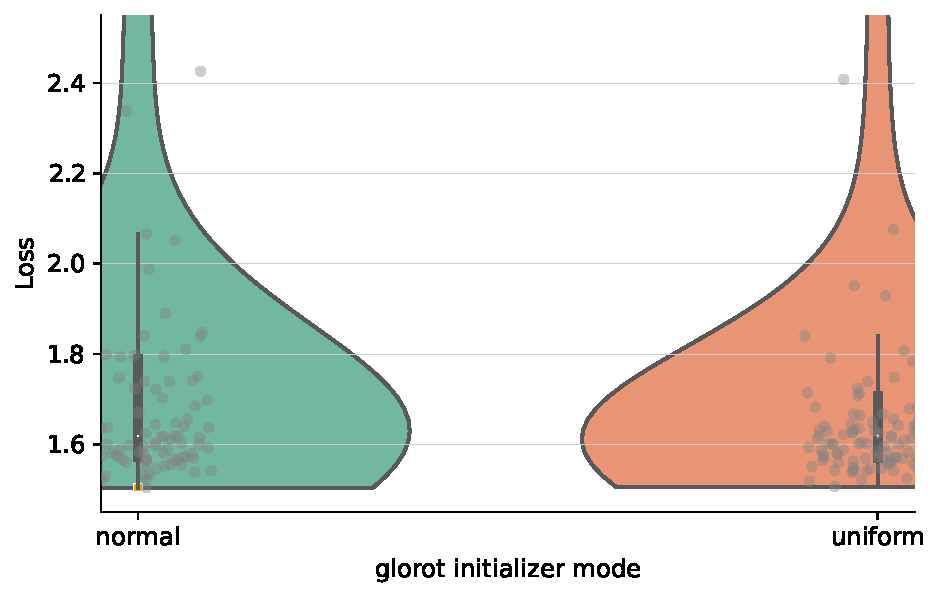
\includegraphics[width=0.48\textwidth]{sec_methodology_hyperopt_plot_initializer.pdf}
                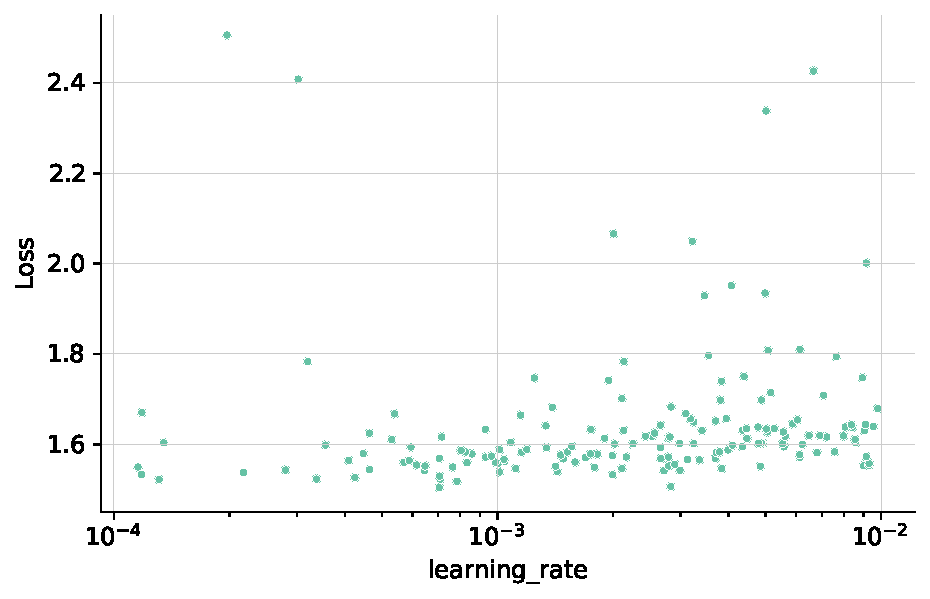
\includegraphics[width=0.48\textwidth]{sec_methodology_hyperopt_plot_lr.pdf} \\
                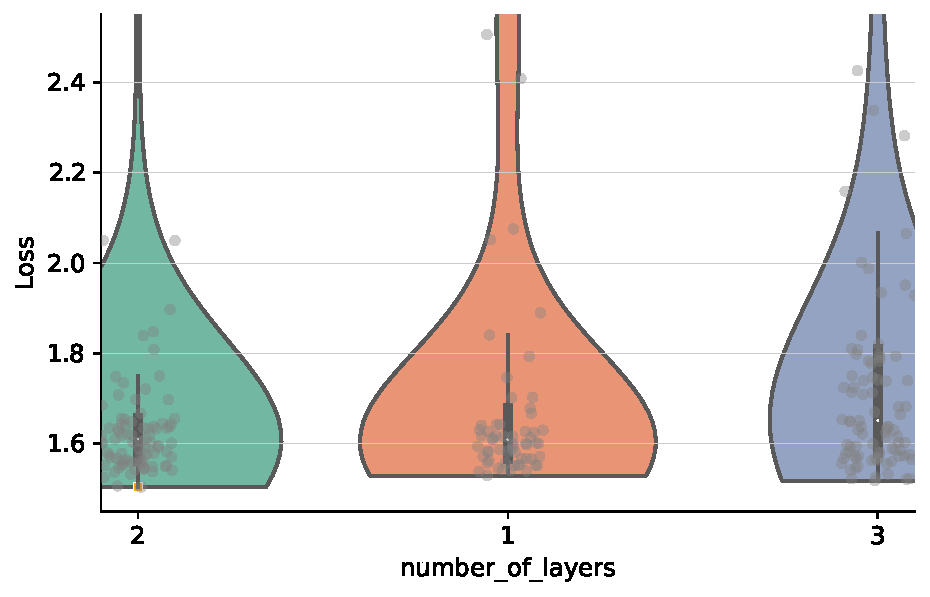
\includegraphics[width=0.48\textwidth]{sec_methodology_hyperopt_plot_number_of_layers.pdf}
                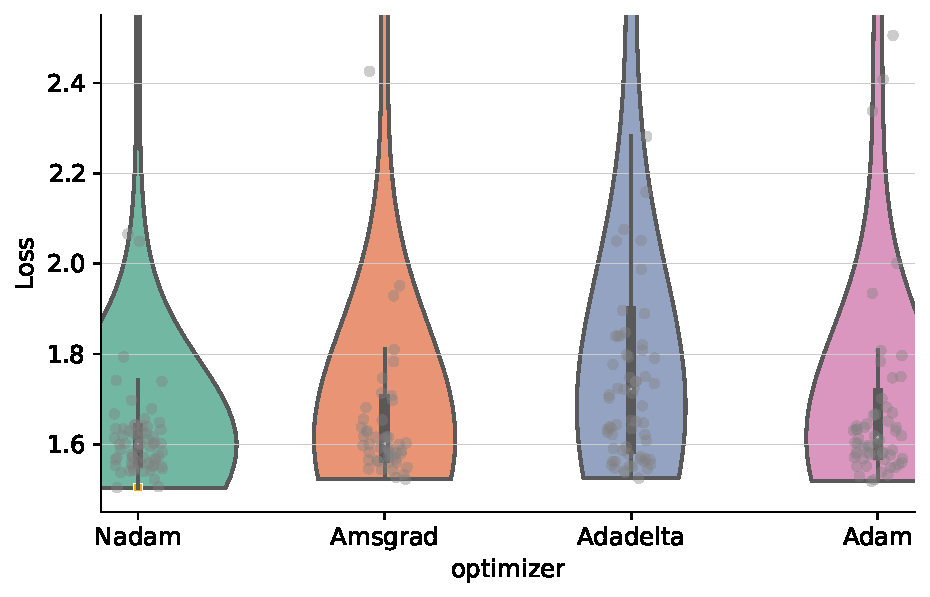
\includegraphics[width=0.48\textwidth]{sec_methodology_hyperopt_plot_optimizers.pdf}
            \end{center}
        \end{column}
    \end{columns}
\end{frame}


\subsection{Phenomenology}


\begin{frame}[t]{High-precision: gluon}
  \begin{equation*}
  \mathcal{L}_{i j}\left(M_{X}, y, \sqrt{s}\right)
  =\frac{1}{s} \sum_{i, j} f_{i}\left(\frac{M_{X} e^{y}}{\sqrt{s}}, M_{X}\right) f_{j}\left(\frac{M_{X} e^{-y}}{\sqrt{s}}, M_{X}\right)
  \end{equation*}
  \begin{center}
    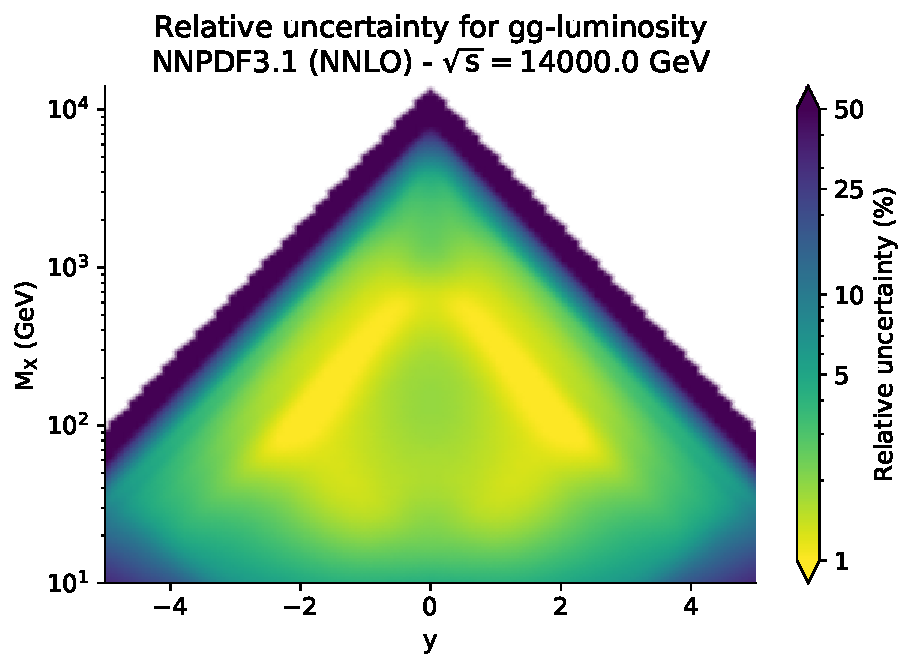
\includegraphics[width=0.4\textwidth]{plot_lumi2d_uncertainty_NNPDF31_gg}
    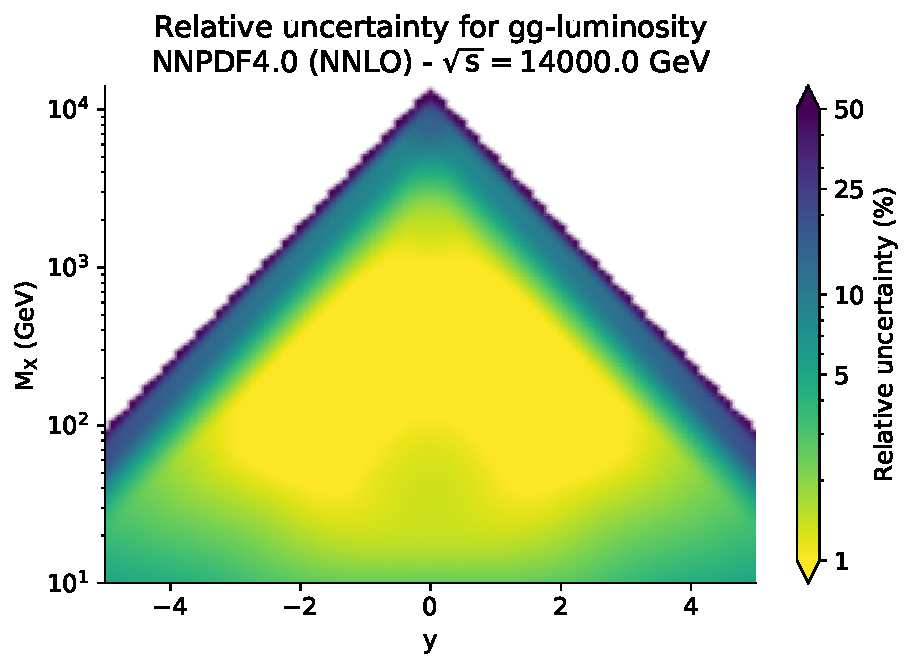
\includegraphics[width=0.4\textwidth]{plot_lumi2d_uncertainty_NNPDF40_gg}
  \end{center}
\end{frame}

\begin{frame}[t]{High-precision: singlet }
  \begin{equation*}
  \mathcal{L}_{i j}\left(M_{X}, y, \sqrt{s}\right)
  =\frac{1}{s} \sum_{i, j} f_{i}\left(\frac{M_{X} e^{y}}{\sqrt{s}}, M_{X}\right) f_{j}\left(\frac{M_{X} e^{-y}}{\sqrt{s}}, M_{X}\right)
  \end{equation*}
  \begin{center}
    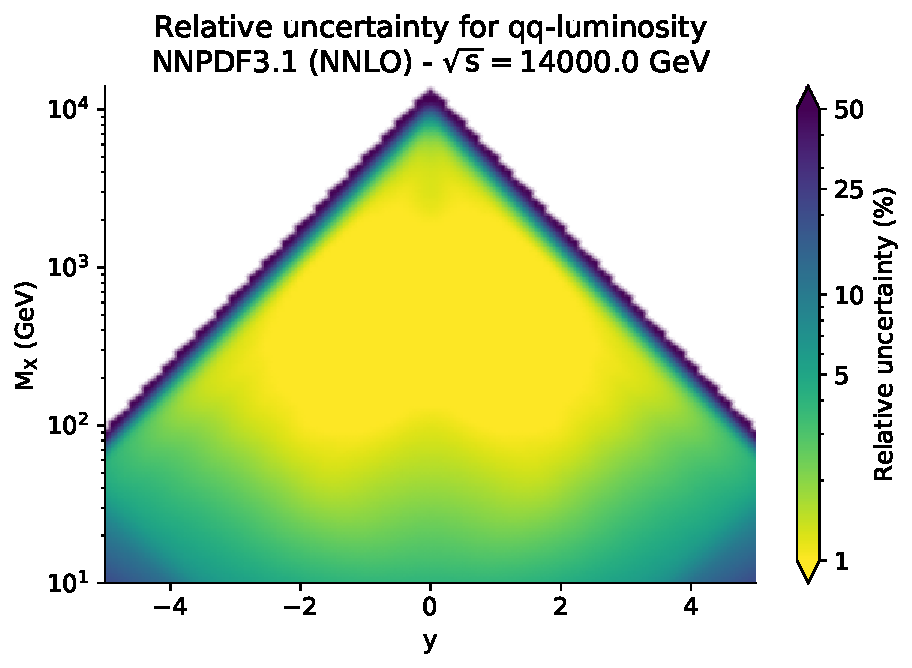
\includegraphics[width=0.4\textwidth]{plot_lumi2d_uncertainty_NNPDF31_qq}
    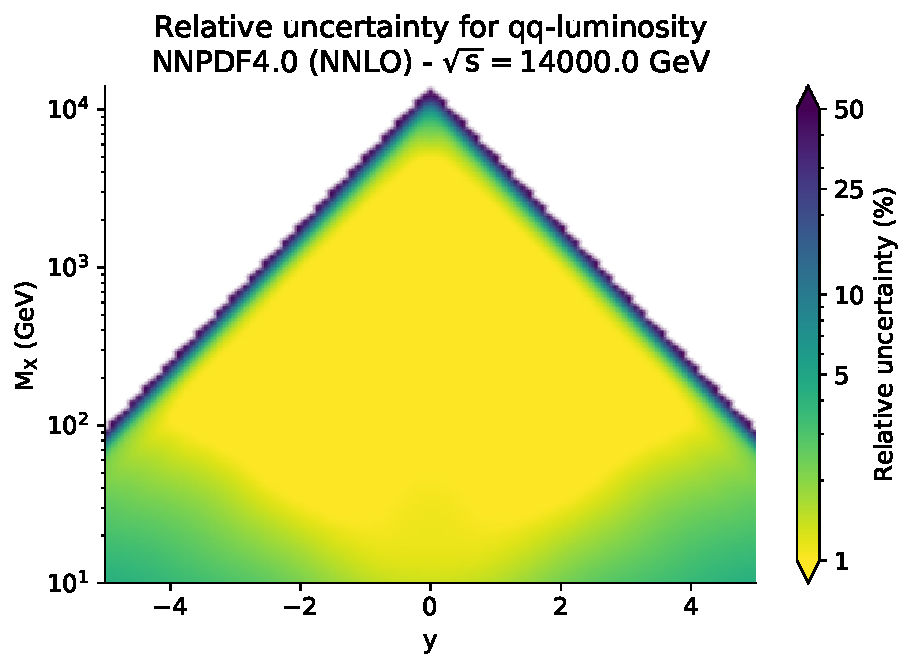
\includegraphics[width=0.4\textwidth]{plot_lumi2d_uncertainty_NNPDF40_qq}\\
  \end{center}
  Typical uncertainties in the data region:
  \begin{itemize}
    \item singlet: from $\sim 3\%$ to $\sim 1\%$
    \item nonsinglet: from $\sim 5\%$ to $\sim 2\%$
  \end{itemize}
\end{frame}


\begin{frame}[t]{Impact of the new data}
  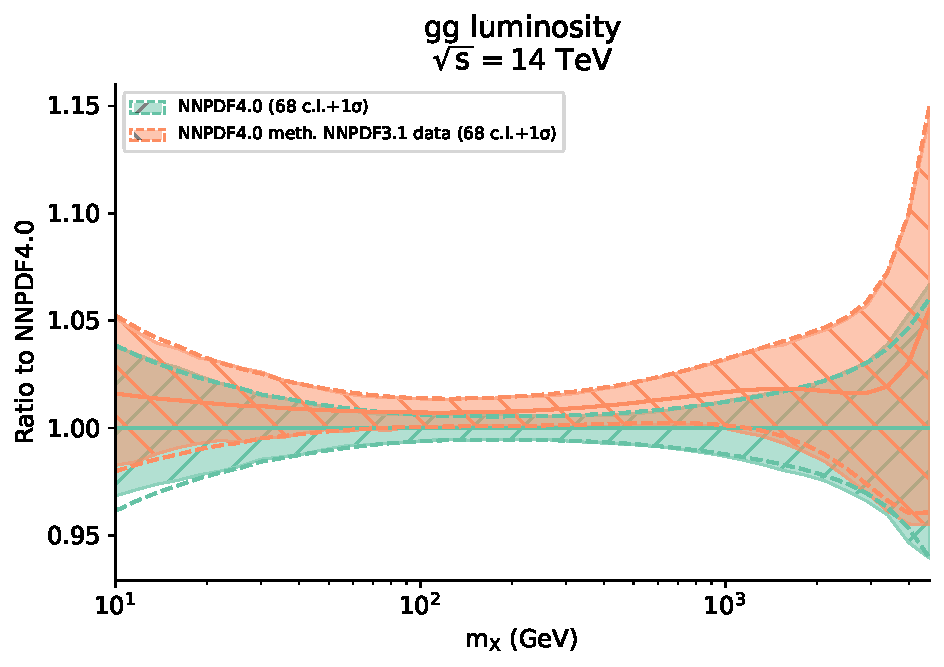
\includegraphics[width=0.45\textwidth]{lumi1d_gg_NNPDF40meth_NNPDF31data}
  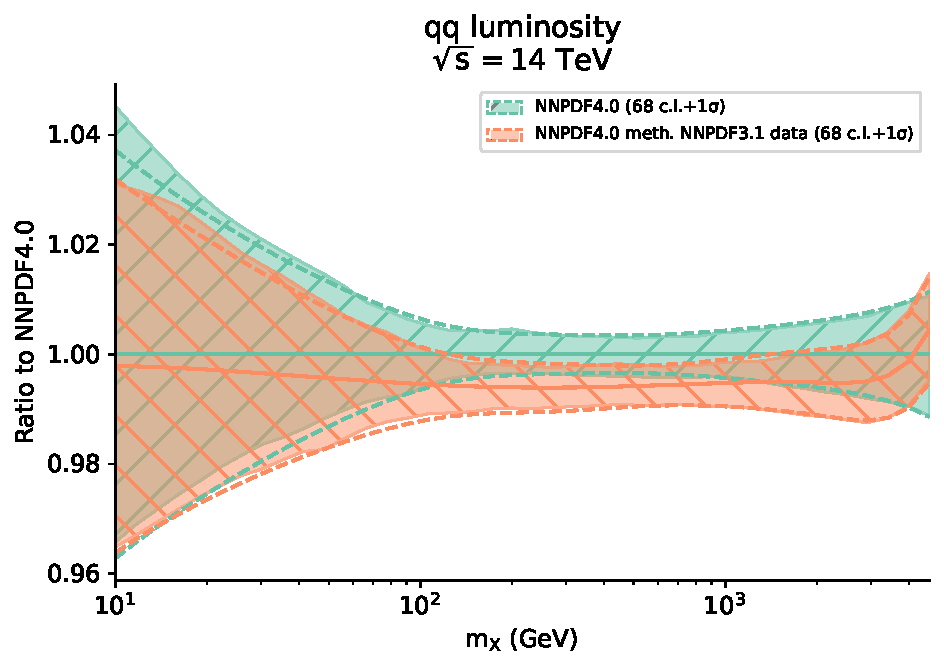
\includegraphics[width=0.45\textwidth]{lumi1d_qq_NNPDF40meth_NNPDF31data}\\
  Individual datasets have a limited impact, but collectively they result in:
  \begin{itemize}
      \item Moderate reduction of PDF uncertainties
      \item Shifts in central value at the one-sigma level
  \end{itemize}
\end{frame}


\begin{frame}[t]{Impact of the new fitting methodology}
  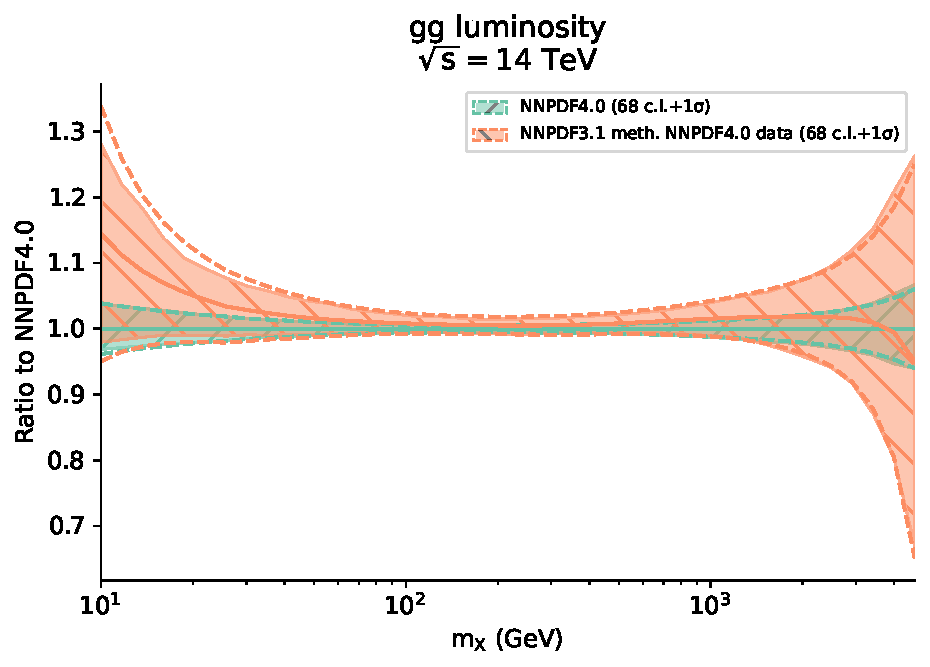
\includegraphics[width=0.45\textwidth]{lumi1d_gg_NNPDF31meth_NNPDF40data}
  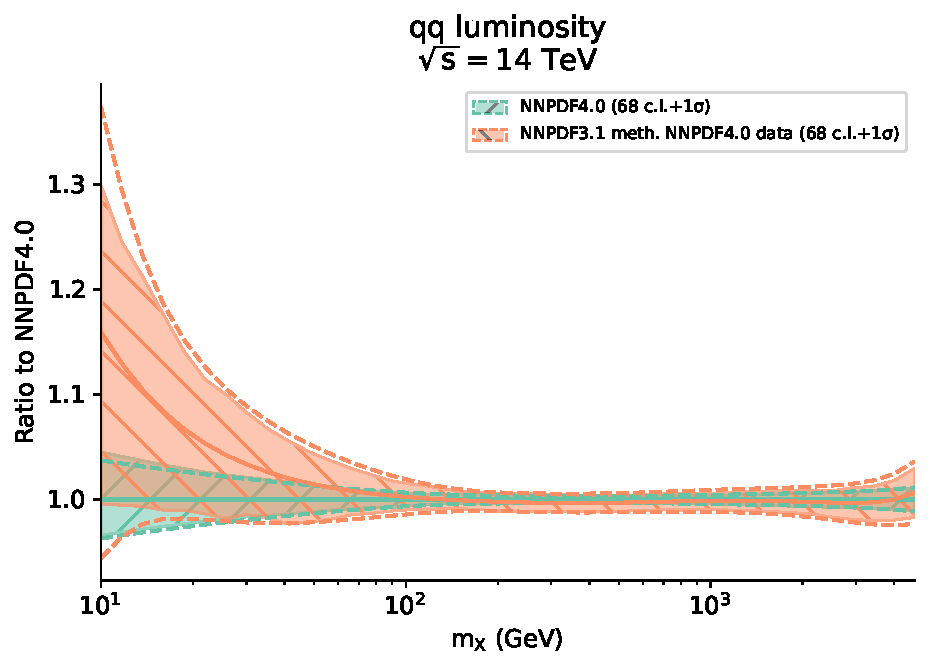
\includegraphics[width=0.45\textwidth]{lumi1d_qq_NNPDF31meth_NNPDF40data}
  \begin{columns}
      \column{0.45\linewidth}
      \begin{itemize}
                \item Significant reduction of PDF uncertainties
            \item Good agreement between the central values
        \end{itemize}
        \column{0.5\linewidth}
            \begin{block}{}
                \fontsize{7}{6}\selectfont
                PDF uncertainties are validated using closure tests and future tests\\
                Validation tests successful for both NNPDF4.0 and NNPDF3.1
            \end{block}
    \end{columns}
\end{frame}

\begin{frame}[t]{The open-source NNPDF code}
  \begin{columns}[T]
    \begin{column}{0.48\textwidth}
      \begin{itemize}
        \item The full NNPDF code has been made public along with user friendly documentation
        \item This includes: fitting, hyperoptimization, theory, data processing, visualization
        \item It is possible to reproduce all results of NNPDF4.0 and more!
      \end{itemize}
    \end{column}
    \begin{column}{0.48\textwidth}
      \centering
      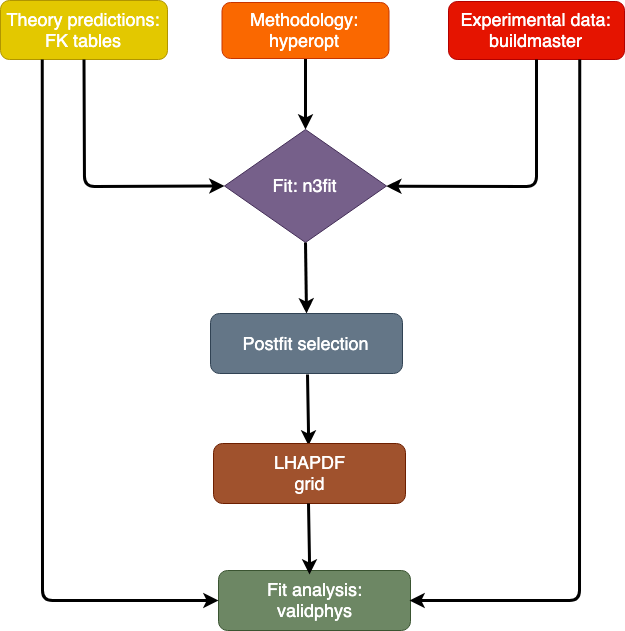
\includegraphics[width=0.65\textwidth]{diagram.png}
    \end{column}
  \end{columns}
    \begin{block}{}
        \centering
    \href{https://link.springer.com/article/10.1140/epjc/s10052-021-09747-9}{Eur.Phys.J.C 81 (2021) 10, 958} \\
    \url{https://github.com/NNPDF/nnpdf} \\
    \url{https://docs.nnpdf.science}
    \end{block}
\end{frame}



%%%%%%%%%%%%%%%%%%%%%%%%%%%%%%%%%%%%%%%%%%%%%%%%%%%%%%%%%%%%%%%%%%%%%%%%%%%%%%%%
{
\AtBeginSection{}
\section{PDF correlations}
\begin{frame}
  \begin{center}
    \usebeamerfont{section title}{PDF correlations}\\
    \vspace*{0.3cm} {\small 2110.08274}
  \end{center}
\end{frame}
}

\begin{frame}[t]{PDF correlations: definition and application}
  \textbf{Definition:}\\[0.3cm]
  Covariance: \\
  $\operatorname{Cov}\left[f_a, f_b\right]\left(x, x^{\prime}\right)=E\left[f_a\left(x, Q_0^2\right) f_b\left(x^{\prime}, Q_0^2\right)\right]-E\left[f_a\left(x, Q_0^2\right)\right] E\left[f_b\left(x^{\prime}, Q_0^2\right)\right]$\\[0.3cm]

  Correlation: \\
  $\rho\left[f_a, f_b\right]\left(x, x^{\prime}\right)=\frac{\operatorname{Cov}\left[f_a, f_b\right]\left(x, x^{\prime}\right)}{\sqrt{\operatorname{Var}\left[f_a\right](x) \operatorname{Var}\left[f_a^q\right]\left(x^{\prime}\right)}}$\\[0.3cm]

  In the MC approach this can be calculated using\\
  $E \left[f_a\left(x, Q_0^2\right) f_b\left(x^{\prime}, Q_0^2\right)\right]=\frac{1}{N} \sum_{r=1}^N f_a^{(r)}\left(x, Q_0^2\right) f_b^{(r)}\left(x^{\prime}, Q_0^2\right)$\\[0.3cm]

  \begin{columns}[t]
    \column{0.6\textwidth}
      Correlation {\bf induced by} data, theory (e.g. sumrules), and methodology (e.g. preprocessing).\\[0.3cm]

      \column{0.39\textwidth}
      \vspace*{-3cm}
      \begin{figure}
        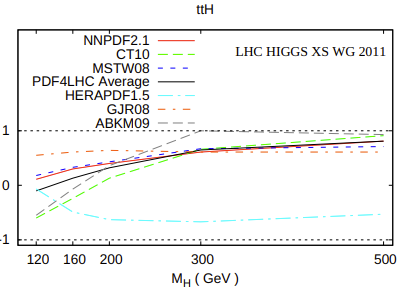
\includegraphics[width=0.89\textwidth]{ggh_tth_correlation.png}
        \caption*{{\bf Application}: determination of PDF induced signal-background correlation between e.g. ggH and ttH}
    \end{figure}
  \end{columns}
\end{frame}

\subsection{Correlation between different sets of PDFs}

\begin{frame}[t]{Correlations between different PDF sets}
  General {\bf cross-covariance} between PDFs in {\bf different sets}, e.g. NNPDF4.0 and MSHT20:
  $$
  \operatorname{Cov}\left[f_a^{\rm NNPDF}, f_b^{\rm MSHT}\right]\left(x, x^{\prime}\right)=E\left[f_a^{\rm NNPDF}\left(x, Q_0^2\right) f_b^{\rm MSHT}\left(x^{\prime}, Q_0^2\right)\right]-E\left[f_a^{\rm NNPDF}\left(x, Q_0^2\right)\right] E\left[f_b^{\rm MSHT}\left(x^{\prime}, Q_0^2\right)\right]
  $$
    \vspace*{0.3cm}
  \begin{columns}[T]
    \begin{column}{0.59\textwidth}
      Special cases of cross-correlation:
      \begin{itemize}
        \item F-correlation - same PDF, different flavor  $\rho\left[f_a^{\rm NNPDF}, f_b^{\rm NNPDF}\right]$
        \item S-correlation - different PDF, same flavor $\rho\left[f_a^{\rm NNPDF}, f_a^{\rm MSHT}\right]$
      \end{itemize}
      % \vspace*{0.3cm}
      \begin{block}{}
        \centering
        {The same replica must be used when calculating covariance}
      \end{block}
      If $f^{(r)}$ and $f^{(r^\prime)}$ are uncorrelated, covariance vanishes: $E\left[f_a f_b\right]=\frac{1}{N} \sum_{r=1}^N f_a^{(r)} f_b^{(r^\prime)}=\left[ f_a\right]\left[ f_b\right]$

      \vspace*{0.3cm}
      {\bf Problem}: What is the meaning of ``same replica'' across PDF sets?
    \end{column}
    \begin{column}{0.39\textwidth}
      \only<2>{
      {\bf Possible solution}: PDF replicas fitted to the same data replica
      \begin{itemize}
        \item Fit $f^{{\rm MSHT}(r)}$ and $f^{{\rm NNPDF}(r)}$ to the same data replica $r$
        \item Calculate covariance as \\ $E \left[f_a f_b\right]=\frac{1}{N} \sum_{r=1}^N f_a^{{\rm NNPDF}(r)} f_b^{{\rm MSHT}(r)}$
      \end{itemize}
      }
    \end{column}
  \end{columns}
\end{frame}



\begin{frame}[t]{Uncorrelated methodological aspects}
  The data replica {\bf does not} uniquely determine the PDF replica
  \begin{columns}
    \begin{column}{0.49\textwidth}
      \begin{figure}
        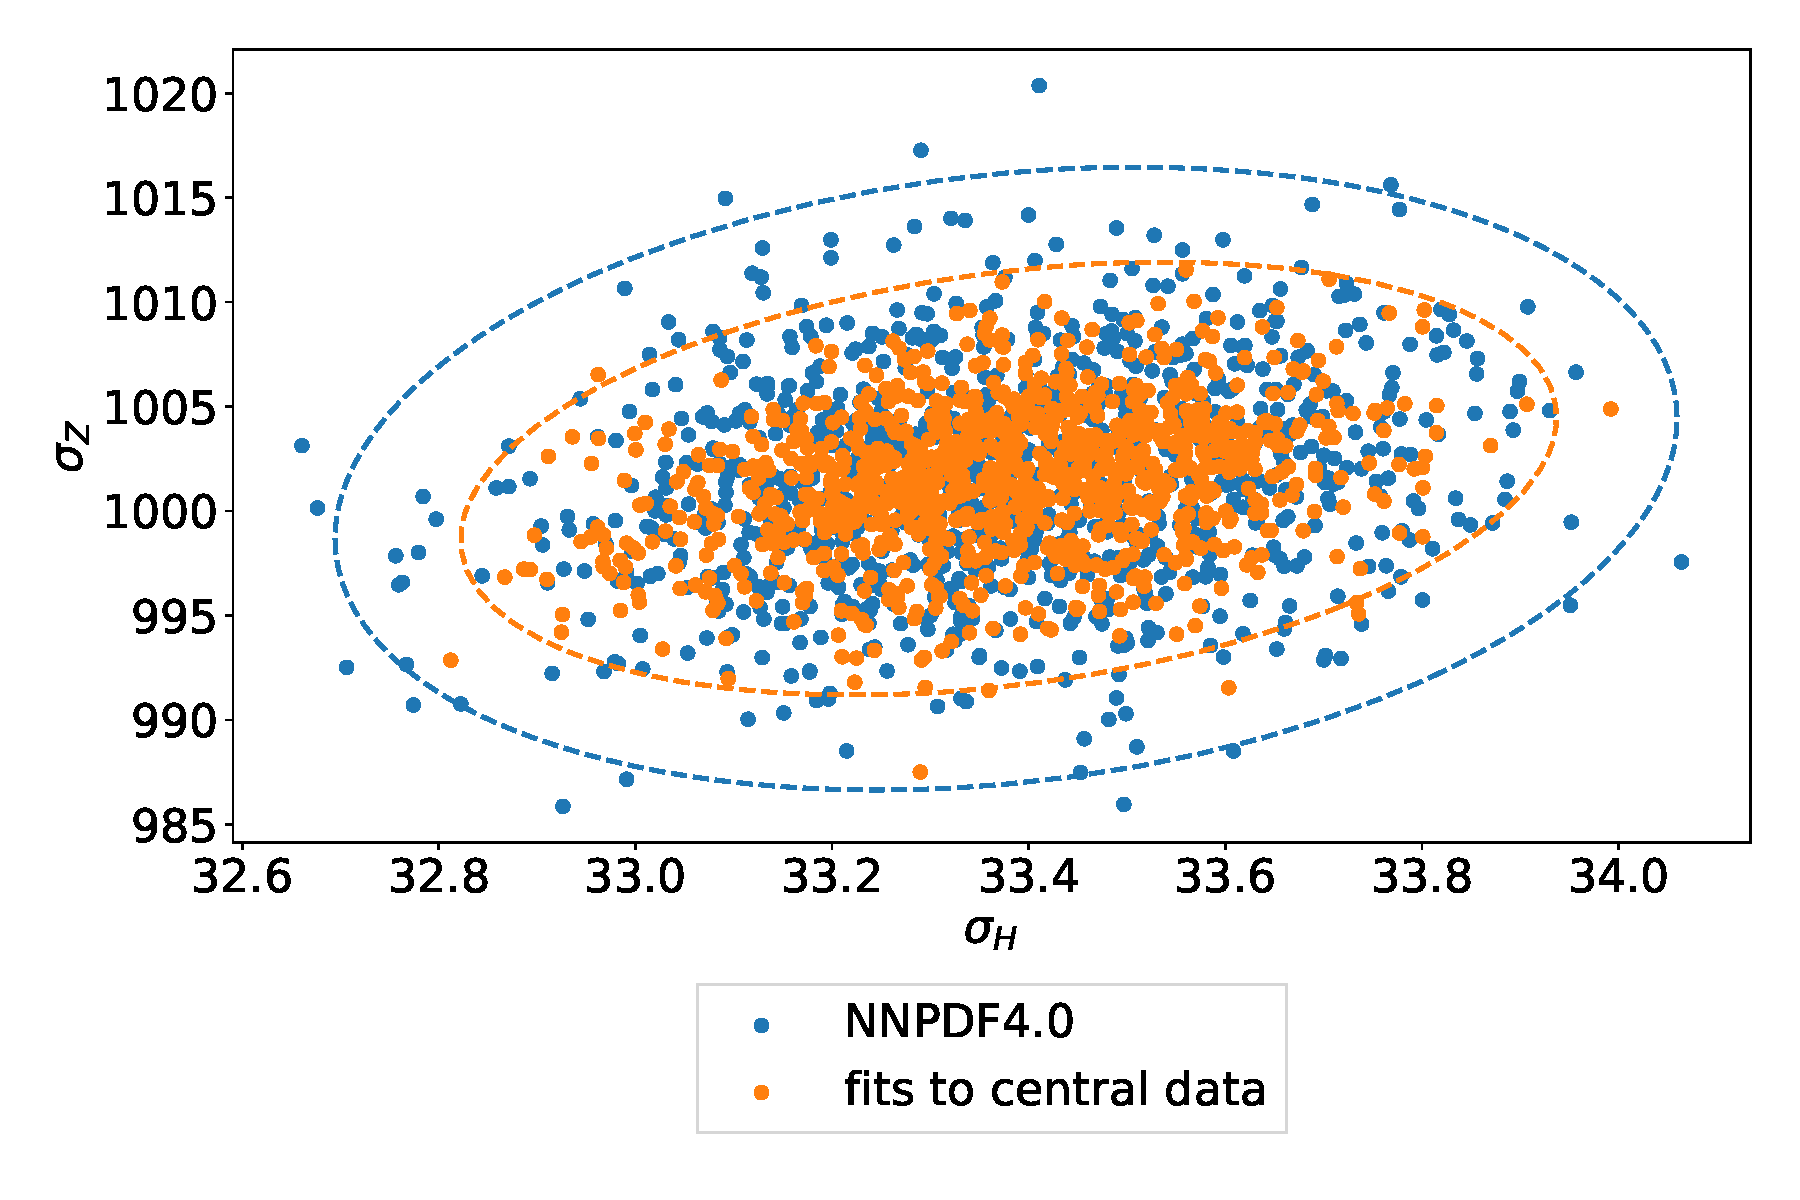
\includegraphics[width=0.9\textwidth]{hopplot_only_3sigma.pdf}
      \end{figure}
    \end{column}
    \begin{column}{0.49\textwidth}
      \only<2>{
      PDF depends on uncorrelated methodological aspects:
      \begin{itemize}
        \item initialization of the neural network
        \item preprocessing exponents
        \item training/validation mask
        \item \ldots
      \end{itemize}
      }
    \end{column}
  \end{columns}
\end{frame}



\begin{frame}[t]{Data-induced correlation}
  Let us distinguish
  \begin{itemize}
    \item data replicas $r$
    \item methodological replicas $r^\prime$
  \end{itemize}
  $$
  \left|\frac{1}{N} \sum_{r=1}^N f_a^{\left(r, r^{\prime}\right)} f_b^{\left(r, r^{\prime \prime}\right)}-E\left[f_a\right] E\left[f_b\right]\right| \leq\left|\frac{1}{N M} \sum_{r=1}^N \sum_{r^{\prime}=1}^M f_a^{\left(r, r^{\prime}\right)} f_b^{\left(r, r^{\prime}\right)}-E\left[f_a\right] E\left[f_b\right]\right|
  $$

  \vspace*{0.3cm}
  Only {\bf data-induced} contributions are calculated
  \begin{figure}
    \centering
    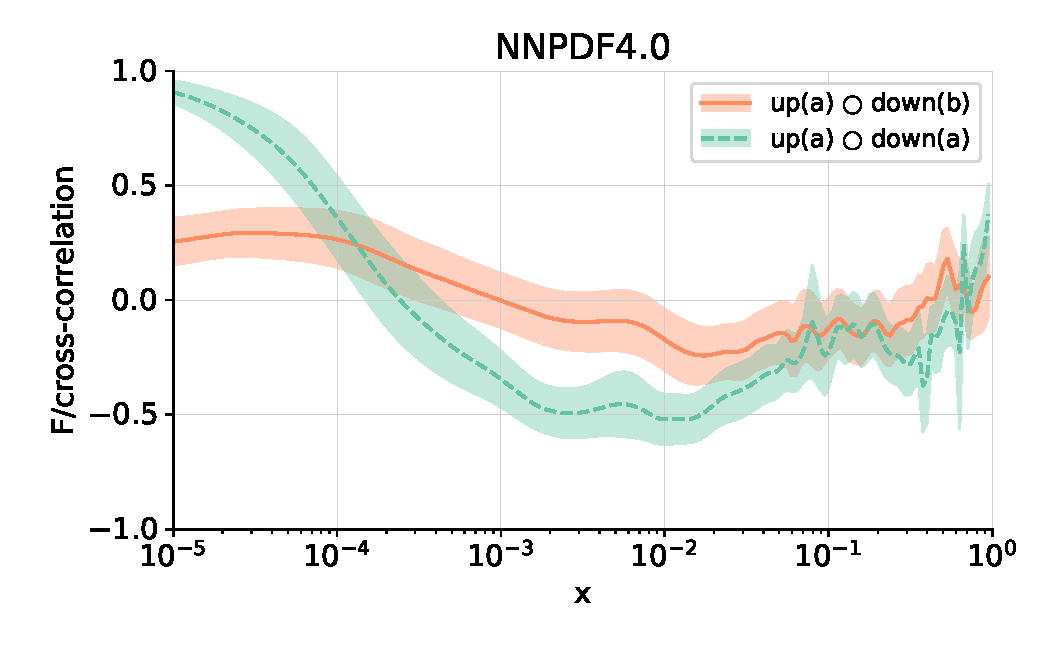
\includegraphics[width=0.45\textwidth]{correlation_upadowna_40.pdf}
  \end{figure}

\end{frame}


\begin{frame}[t]{Correlated methodological replicas}
  \begin{itemize}
    \item Can easily be done for {\bf parametric} components such as preprocessing or architecture
    \item Noticeable impact of {\bf preprocessing}, negligible for {\bf architecture}
  \end{itemize}

  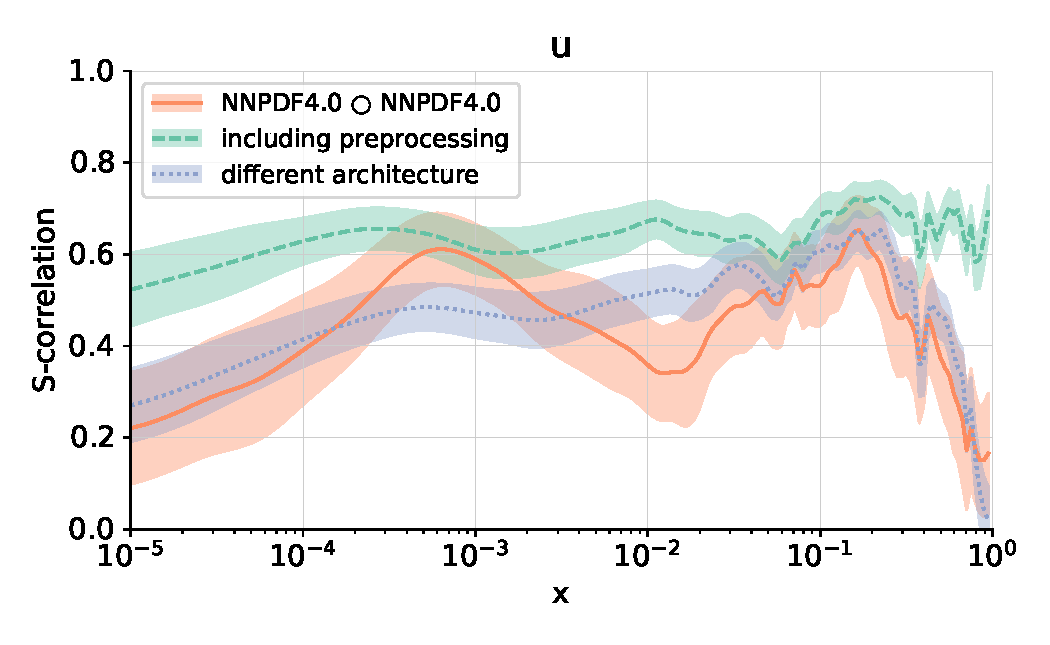
\includegraphics[width=0.49\textwidth]{correlation_2.pdf}
  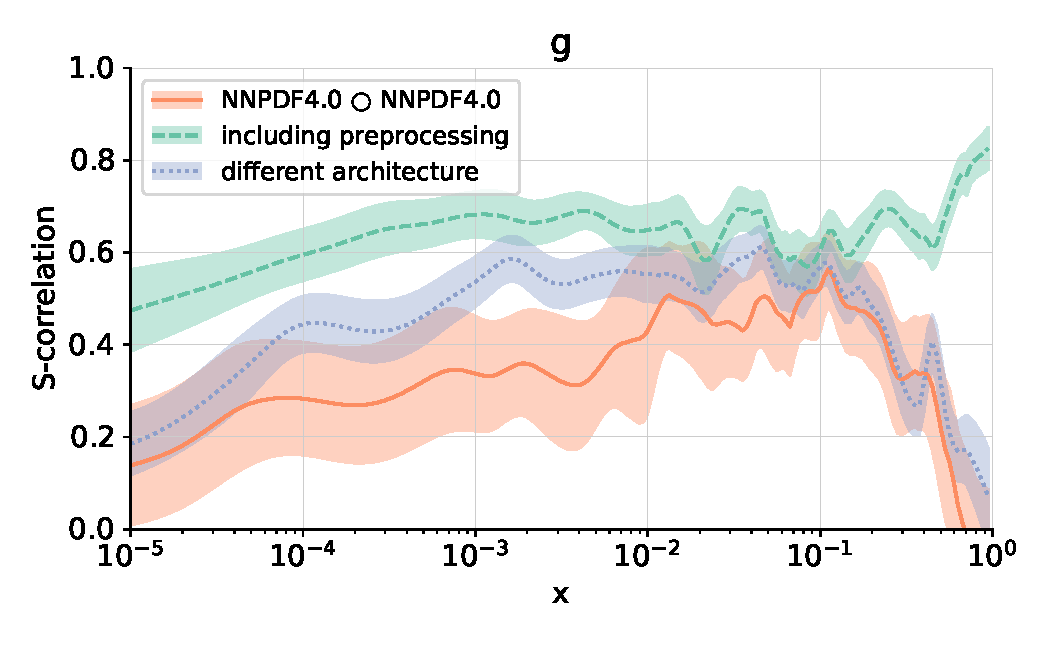
\includegraphics[width=0.49\textwidth]{correlation_21.pdf}

  \noindent\makebox[\textwidth][c] correlation is due to uncorrelated aspects of the methodology
    \item<2> Calculate {\bf correlation between different methodologies}
    \item<2> "weakest link" NNPDF3.1$\circ$NNPDF4.0 $\approx$ NNPDF3.1$\circ$NNPDF3.1
  \end{itemize}
  \only<2>{
    \begin{block}{}
      {Higher correlation indicates a more efficient methodology}
    \end{block}
  }
  \begin{figure}
    \centering
    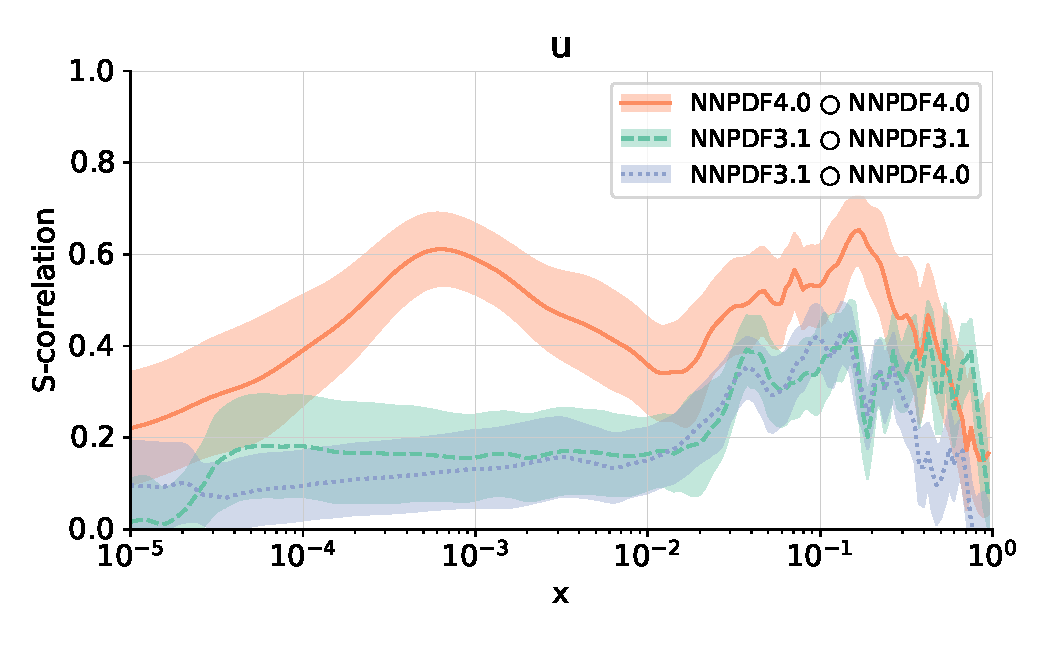
\includegraphics[width=0.4\textwidth]{correlation1_2.pdf}
    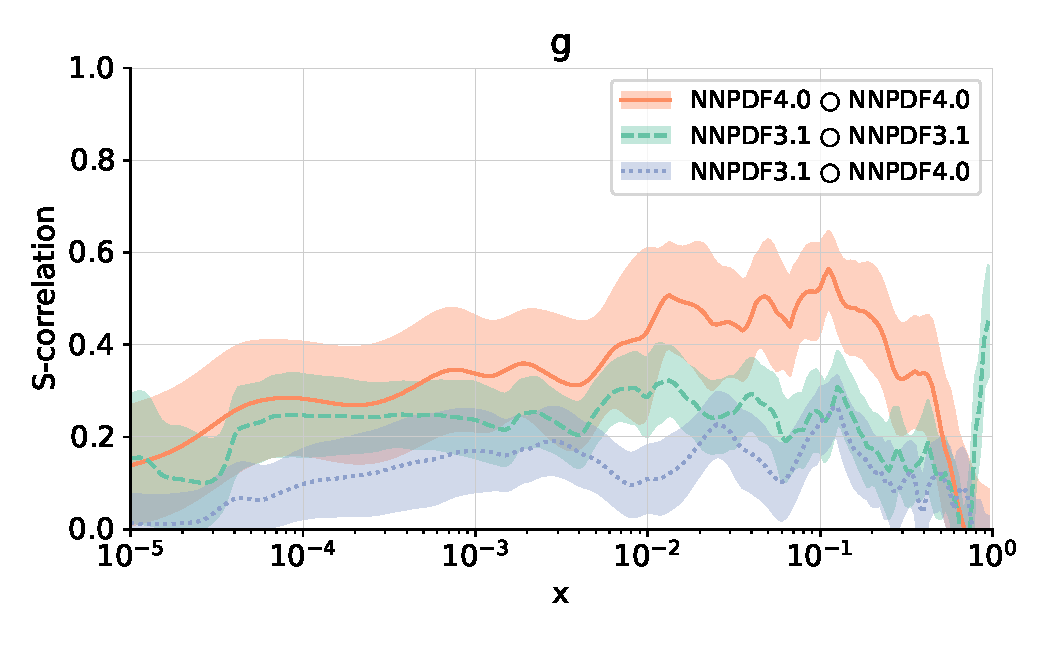
\includegraphics[width=0.4\textwidth]{correlation1_21.pdf}
  \end{figure}

\end{frame}


\subsection{Combination of PDF sets}


\begin{frame}[t]{PDF4LHC combination}
  \vspace*{-1cm}
      \hfill 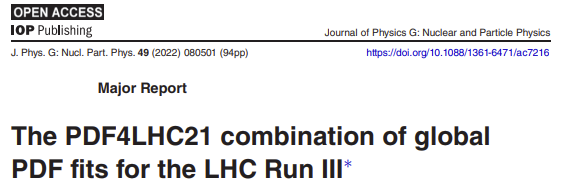
\includegraphics[width=0.35\textwidth]{pdf4lhc21_screenshot.png}
      \vspace*{-0.3cm}
      \begin{itemize}
        \item All PDFs assumed to have {\bf equal probability}
        \item {\bf Monte Carlo combination} of 300 replicas from each of the underlying PDF sets
      \end{itemize}


      \begin{figure}
        \centering
        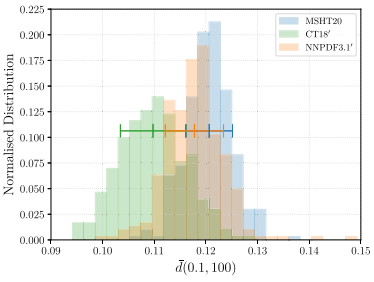
\includegraphics[width=0.3\textwidth]{pdf4lhc_combination_dbar.png}
      \end{figure}
      {\bf Uncertainty} of the Monte Carlo combination:\\
      $
      {\rm Var}[f_a^{\rm comb}] = \frac{1}{2}\left({\rm Var}[f_a^{\rm MSHT}] +{\rm Var}[f_a^{\rm NNPDF}]  \right)+  \frac{1}{4} (E\left[f_a^{\rm MSHT}\right] - E\left[f_a^{\rm NNPDF}\right])^2
      $

      {\bf combined uncertainty bigger} than average uncertainty if central values disagree
\end{frame}


\begin{frame}[t]{Correlated PDF combination?}

  \begin{columns}[t]
    \column{0.59\textwidth}
    {\bf Idea:}
    \begin{itemize}
      \item Combine PDF determinations as independent observations
      \item Correlated combination produces a {\bf weighted average}
    \end{itemize}
      Assuming two sets of same variance, $\mathrm{Var}[f_a^{\rm NNPDF}] = \mathrm{Var}[f_a^{\rm MSHT}]$:
      $$
      \mathrm{Var}[f_a^{\rm comb}] = \frac{1}{2}\left(1+\rho[f_a^{\rm MSHT},f_a^{\rm NNPDF}]\right)\mathrm{Var}[f_a^{\rm NNPDF}]
      $$

      \only<2->{
      {\bf Problems:}
      \begin{itemize}
        \item Does not account for difference in central values
        \item How to compute correlations reliably? I.e. methodological components
      \end{itemize}
      \begin{block}{}
        {Underestimated data-induced correlations leads to {\bf underestimated uncertainty of combination}}
      \end{block}
      }
    \column{0.39\textwidth}
      \only<3>{What if we combine many repeated determinations of the same PDF set?}
      \begin{center}
        \only<2>{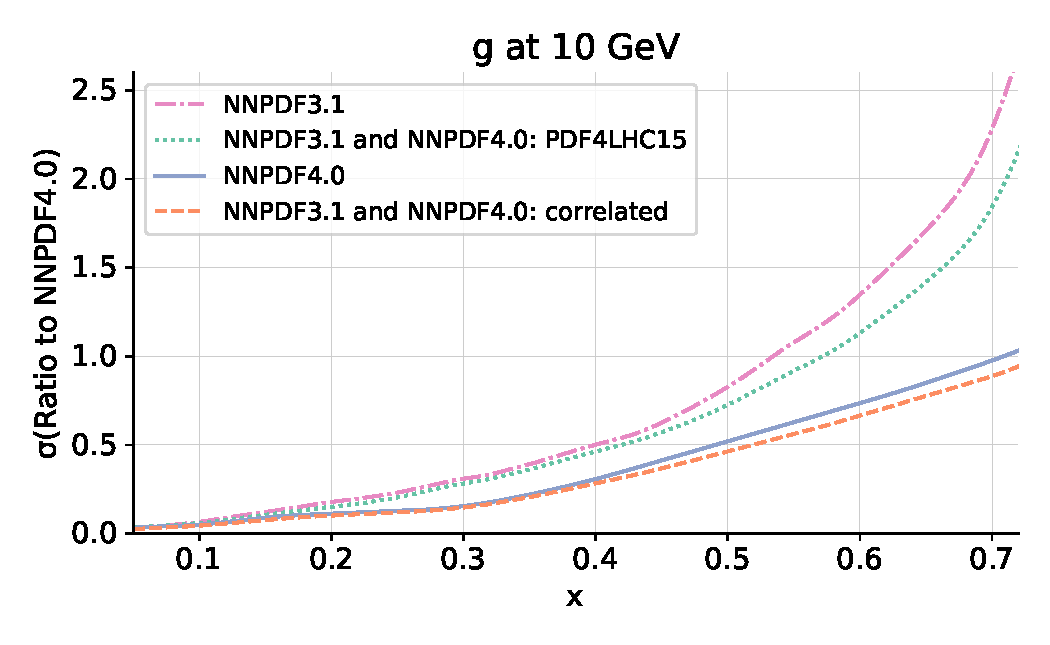
\includegraphics[width=\textwidth]{gluon34.pdf}}
        \only<3>{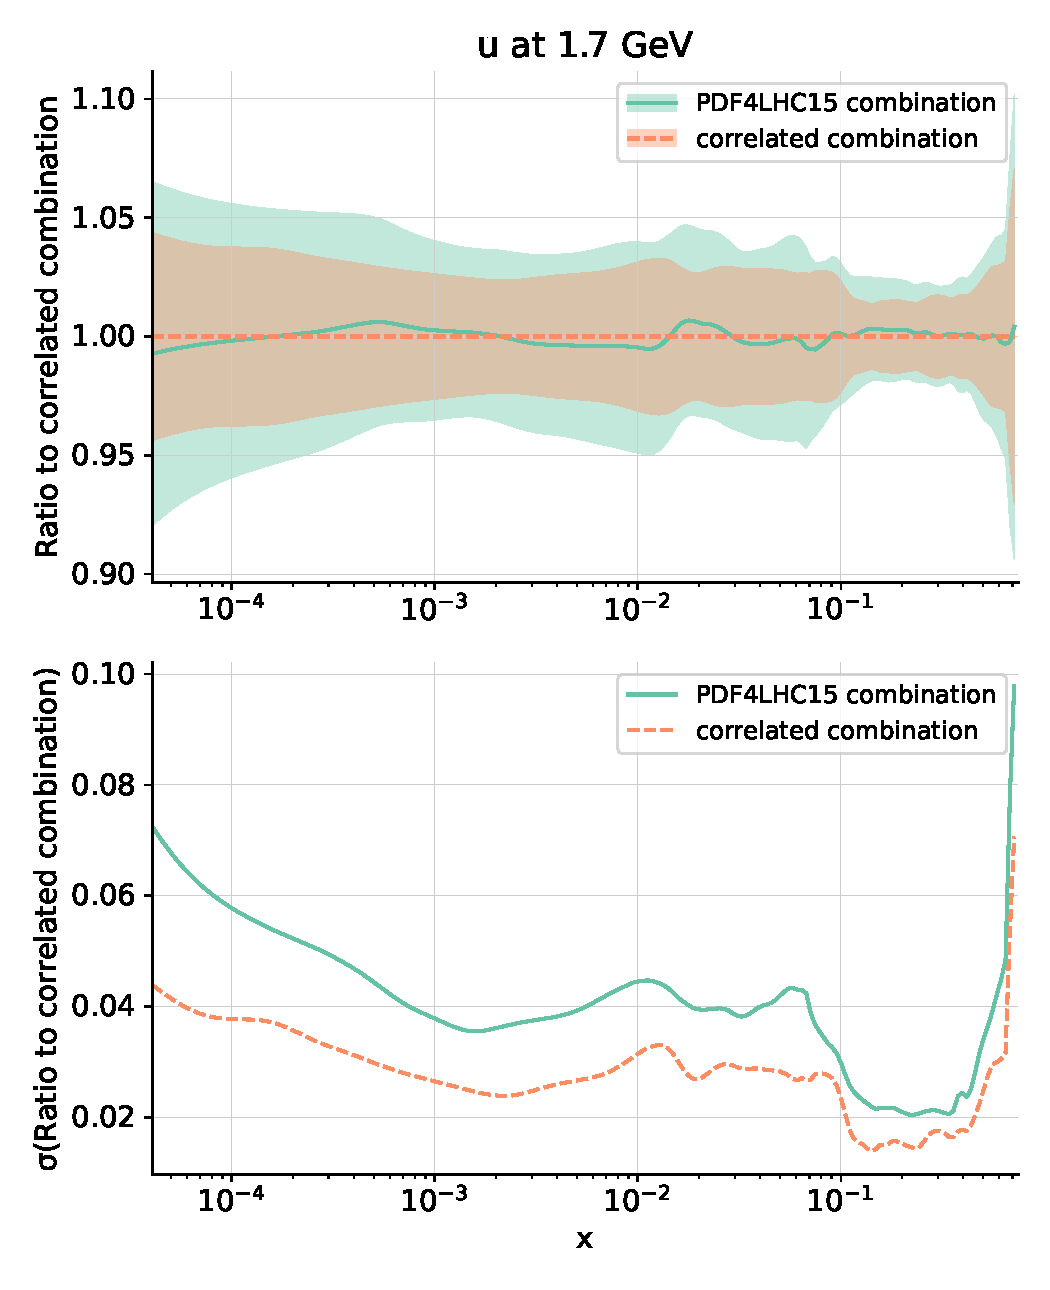
\includegraphics[width=0.7\textwidth]{ratio_2.pdf}}
      \end{center}
  \end{columns}
\end{frame}


%%%%%%%%%%%%%%%%%%%%%%%%%%%%%%%%%%%%%%%%%%%%%%%%%%%%%%%%%%%%%%%%%%%%%%%%%%%%%%%%
{
\AtBeginSection{}
\section{Future ML developments}
\begin{frame}
  \begin{center}
    \usebeamerfont{section title}{Future ML developments}\\
    \vspace*{0.3cm} {\small 2111.02954 and 2211.12961}
  \end{center}
\end{frame}
}

\subsection{A data-based parametrization}

\begin{frame}[t]{Preprocessing}
  \begin{itemize}
    \item PDF model: $f_a=A_ax^{\alpha_a}(1-x)^{\beta_a} \mathrm{NN}_a(x,\log x)$
    \item Exponents $\alpha_a$ and $\beta_a$ sampled {\bf randomly} per replica
    \item Range determined through {\bf self-consistent iterative procedure}
    \item $x$ and $\log x$ inputs
  \end{itemize}

  \begin{center}
    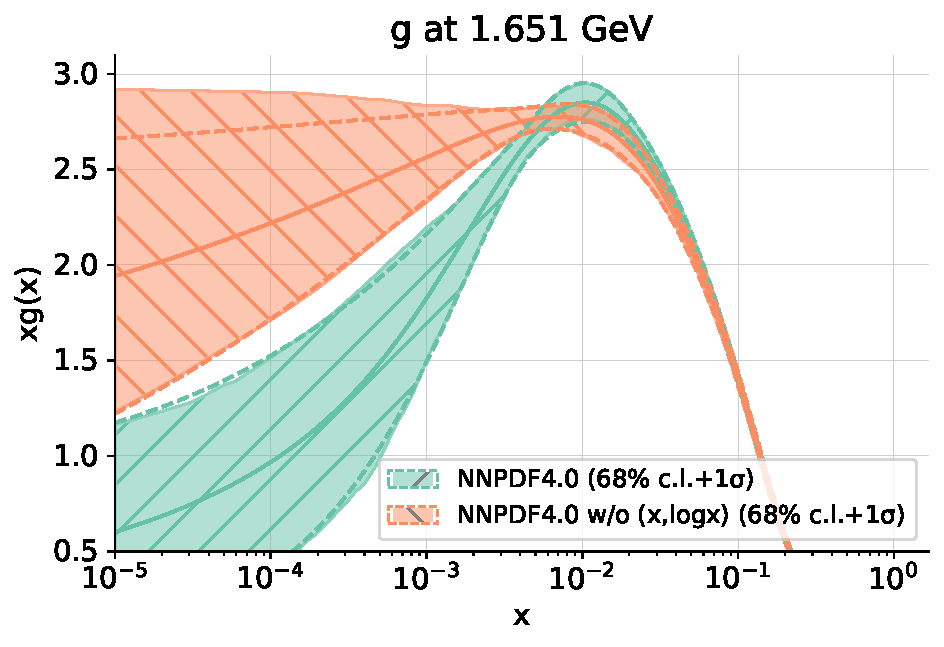
\includegraphics[width=0.39\textwidth]{pdf_g_without_xlogx.pdf}
  \end{center}

  \vspace*{-1cm}
  \begin{itemize}
    \item Need to {\bf iterate}
    \item Hierarchy in input scale. A source of {\bf bias?}
    \item Sampled exponents add {\bf noise} during hyperopt
  \end{itemize}
\end{frame}

\begin{frame}[t]{Feature scaling}
  \vspace*{-0.5cm}
  \begin{columns}
    \begin{column}{0.33\textwidth}
      \begin{figure}
        \includegraphics[width=0.8\textwidth]{default_xgrid.pdf}
        \vspace*{-0.3cm}
        \caption*{$x$}
      \end{figure}
    \end{column}
    \begin{column}{0.33\textwidth}
      \begin{figure}
        \includegraphics[width=0.8\textwidth]{log_xgrid.pdf}
        \vspace*{-0.3cm}
        \caption*{$\log x$}
      \end{figure}
    \end{column}
    \begin{column}{0.33\textwidth}
      \begin{figure}
        \includegraphics[width=0.8\textwidth]{ecdf_xgrid.pdf}
        \vspace*{-0.3cm}
        \caption*{eCDF($x$)}
      \end{figure}
    \end{column}
  \end{columns}

  Avoid potential bias:
  \begin{itemize}
    \item generate flat distribution: effective cumulative distribution function (eCDF)
    \item Add interpolation
    \item Rerun hyperopt
    \item[$\Rightarrow$] Only single input
    \item[$\Rightarrow$] No preprocessing needed
  \end{itemize}

  \only<2>{
  \begin{minipage}{0.3\textwidth}
    \begin{block}{}
      { Good agreement between NNPDF4.0 and feature scaling!}
    \end{block}
  \end{minipage}

  \vspace*{-2.5cm}
  \begin{center}
    \hspace*{4cm}
    \includegraphics[width=0.32\textwidth]{pdf_u_log.pdf}
    \includegraphics[width=0.32\textwidth]{pdf_gluon_log_feature_vs_nnpdf40.pdf}
  \end{center}
  }
\end{frame}



% \subsection{Automated selection of hyperoptimization k-folds} % maybe not since this is juans work

\subsection{An overfitting metric}


\begin{frame}[t]{Overfitting in hyperopt}

  \begin{itemize}
    \item Statistical fluctuations affecting hyperopt results
    \item Hyperopt solutions can be overfitted or underfitted
  \end{itemize}

  \begin{center}
    \includegraphics[width=0.32\textwidth]{clipnorm_fit_charm_plot_pdfs_c.pdf}
    \vspace*{0.3cm}
    \includegraphics[width=0.32\textwidth]{NNPDF40_fit_charm_plot_pdfs_c.pdf}
  \end{center}

  \begin{itemize}
    \item What does it mean for a PDF to be overfitted?
    \item More wiggles $\to$ overfitting?
    \item More wiggles $\to$ better agreement to data
  \end{itemize}
\end{frame}


\begin{frame}[t]{overfitting metric}
  Validation data only used for early stopping
  \begin{enumerate}
    \item Take set of PDF replicas
    \item Calculated expected validation loss
    \item Compare to real validation loss
  \end{enumerate}
  $$
  \mathcal{R}_O=\chi_\mathrm{val,r}^2\left[\mathcal{T}\left[f^{(r)}\right], \mathcal{D}^{(r)}\right] -  \frac{1}{N}\sum_{r'=1}^{N}\chi_\mathrm{val,r}^2\left[\mathcal{T}\left[f^{(r)}\right], \mathcal{D}^{(r')}\right].
  $$

  Negative $\mathcal{R}_O$ $\to$ overfitting

  \only<2>{
  \begin{figure}
    \begin{subfigure}{0.32\textwidth}
      \includegraphics[width=\textwidth]{clipnorm_fit_charm_plot_pdfs_c.pdf}
      \caption*{old candidate: $\mathcal{R}_O = -0.024\pm 0.012$}
    \end{subfigure}
    \vspace*{0.3cm}
    \begin{subfigure}{0.32\textwidth}
      \includegraphics[width=\textwidth]{NNPDF40_fit_charm_plot_pdfs_c.pdf}
      \caption*{NNPDF4.0: $\mathcal{R}_O = -0.001\pm 0.013$}
    \end{subfigure}
  \end{figure}
  }
\end{frame}


\begin{frame}[t]{}

  {\bf I did not discuss other sources of uncertainty}
  \begin{itemize}
    \item Theory and missing higher order uncertainties (Andrea, next days)
    \item The negligible impact of data inconsistencies (see 2212.07703)
    \item Future tests and closure tests
  \end{itemize}
  \vspace*{0.3cm}
  {\bf Possible future directions}
  \begin{itemize}
    \item Optimize hyperopt folds
    \item Overfitting metric in hyperopt
    \item Parallelization on GPU
    \item Understanding PDF fitting in a Bayesian framework
  \end{itemize}
  More work still to be done!
  \vspace*{2em}
  \only<2>{
  \begin{center}
      {\Large \textbf{Thank you!}}
  \end{center}
  }
\end{frame}


%%%%%%%%%%%%%%%%%%%%%%%%%%%%%%%%%%%%%%%%%%%%%%%%%%%%%%%%%%%%%%%%%%%%%%%%%%%%%%%%
% {
% \AtBeginSection{}
% \section{Neutrino inelastic structure functions}
% \begin{frame}
%   \begin{center}
%     \usebeamerfont{section title}{Neutrino inelastic structure functions}
%   \end{center}
% \end{frame}
% }




\begin{frame}{Determination of the photon PDF}
  \begin{columns}[T]
    \begin{column}{0.59\textwidth}
      Initially the photon PDF has been determined in different ways:
      \begin{itemize}
        \item physical model: sensitive to underlying model
        \item fitting: data does not provide strong constraints
      \end{itemize}

      \vspace*{0.5em}
      However with the LUXqed approach it can be computed perturbatively \\
      based on the observation that the heavy-lepton production cross-section can be written in two ways:
      \begin{itemize}
        \item in terms of structure functions $F_2$, $F_L$
        \item in terms of PDFs (including the photon)
      \end{itemize}

      \vspace*{0.5em}
      luxQED result {\color{gray}\small[Manohar, Nason, Salam, Zanderighi: 1607.04266, 1708.01256]}:
      \vspace*{-0.8em}
      \begin{equation*}
        \begin{split}
          & x \gamma(x, \mu^2)
          =
          \frac{2}{\alpha (\mu^2)} \int\limits_x^1 \frac{dz}{z}
          \Biggl\{ \int_{m_p^2x^2 \over 1-z}^{\mu^2 \over 1-z} \frac{dQ^2}{Q^2}
          \alpha^2(Q^2) \Biggl[ -z^2 F_L(x/z, Q^2) \\
          & + \left( z P_{\gamma q}(z) + \frac{2 x^2 m_p^2}{Q^2} \right)
          F_2(x/z, Q^2)\Biggr] - \alpha^2(\mu^2) z^2 F_2(x/z, \mu^2)\Biggr\}
        \end{split}
      \end{equation*}
    \end{column}

    \begin{column}{0.39\textwidth}
      \vspace*{-2.5em}
      \begin{figure}
        \includegraphics[width=0.89\textwidth]{figures/dataluxqed.png}
        \caption*{Input to construct $F_2$ and $F_L$}
        \includegraphics[width=0.89\textwidth]{figures/luxQED_uncs.png}
        \caption*{Sources of uncertainty}
      \end{figure}
    \end{column}
  \end{columns}
\end{frame}


\begin{frame}{LUXqed PDF determinations}
  LUXqed has been used in all of the most recent QED PDFs:
  \begin{itemize}
      \item LUXqed\_plus\_PDF4LHC15 {\color{gray}\small [1607.04266]}
      \item LUXqed17\_plus\_PDF4LHC15 {\color{gray}\small [1708.01256]}
      \item MMHT2015qed {\color{gray}\small [1907.02750]}
      \item NNPDF3.1luxQED {\color{gray}\small [1712.07053]}
      \item CT18lux and CT18qed {\color{gray}\small [2106.10299]}
      \item MSHT20QED {\color{gray}\small [2111.05357]}
      \item MSHT20qed\_an3lo {\color{gray}\small [2312.07665]}
      \item NNPDF4.0QED {\color{gray}\small [2401.08749 ]}
  \end{itemize}
\end{frame}

% \begin{frame}{Results: photon PDF and luminosity}
%   \begin{center}
%     \includegraphics[width=0.3\textwidth]{figures/photon_comparison.pdf}
%     \includegraphics[width=0.3\textwidth]{figures/pp_lumi_comparison.png}
%     \includegraphics[width=0.3\textwidth]{figures/gp_lumi_comparison.pdf}
%   \end{center}
%   \begin{itemize}
%     \item Because all groups use the luxQED formalism, the photon PDFs agree at percent level
%     \item Luminosity generally in agreement, but differ at very small and very large invariant mass
%   \end{itemize}
% \end{frame}


% ============================================================================


\begin{frame}{Incomplete higher order uncertainties covmat}
  \begin{itemize}
    \item We construct an IHOU matrix following a similar approach by varying the subleading functions
    \item IHOU are independent of MHOU so the uncertainties are added in quadrature
    $$C = C_\mathrm{exp}+C_\mathrm{MHOU}+C_\mathrm{IHOU}$$
  \end{itemize}

  \begin{columns}
    \begin{column}{0.49\textwidth}
      \begin{figure}[!t]
        \centering
        \includegraphics[width=.9\textwidth]{figures/diag_cov_dis_ihou.pdf}
        \caption*{IHOU have a large effect on small-$x$, low-$Q$ DIS data
        }
      \end{figure}
    \end{column}
    \begin{column}{0.49\textwidth}
      \begin{figure}[!t]
        \centering
        \includegraphics[width=.9\textwidth]{figures/diag_cov_dy_ihou_3pt_mhou.pdf}
        \caption*{NNLO MHOU included where N3LO not available \\
          MHOU can similar magnitude as the experimental uncertainty
        }
      \end{figure}
    \end{column}
  \end{columns}


\end{frame}

% \begin{frame}{Magnitude of theory uncertainties}
% % show that for certain processes th unc is of same size as exp unc.
% \end{frame}

% ============================================================================

\begin{frame}{Impact of MHOUs at N3LO}
  \begin{figure}[!t]
    \centering
    \includegraphics[width=0.45\textwidth]{figures/gg_plot_lumi1d.pdf}
    \includegraphics[width=0.45\textwidth]{figures/qqbar_plot_lumi1d.pdf}
  \end{figure}
  \begin{itemize}
    \item Non-negligible impact of MHOUs even at N3LO
    \item[$\Rightarrow$] reason to include exact N3LO calculations for hadronic processes
  \end{itemize}
\end{frame}


% \begin{frame}{Comparison to MSHT20}
%   \begin{figure}[!t]
%     \centering
%     \includegraphics[width=0.45\textwidth]{figures/gg_plot_lumi1d_msht20.pdf}
%     \includegraphics[width=0.45\textwidth]{figures/qqbar_plot_lumi1d_msht20.pdf}
%   \end{figure}
%   \begin{itemize}
%     \item Good agreement with MSHT20 for the quark luminosities
%     \item Also for gluon luminosities, except around the Higgs mass and high-mass
%     \item Similar data but different methodology (including splitting function parametrization)
%   \end{itemize}
% \end{frame}



\end{document}
